%%%%%%%%%%%%%%%%%%%%%%%%%%%%%%%%%%%%%%%%%
%  Design Documentation for CSEE4840
%  Objetive: Explain what I did and how, so someone can continue with the investigation
%
% Important note:
% Chapter heading images should have a 2:1 width:height ratio,
% e.g. 920px width and 460px height.
%
%%%%%%%%%%%%%%%%%%%%%%%%%%%%%%%%%%%%%%%%%

%----------------------------------------------------------------------------------------
%	PACKAGES AND OTHER DOCUMENT CONFIGURATIONS
%----------------------------------------------------------------------------------------

\documentclass[twoside,12pt,fleqn]{book} % Default font size and left-justified equations


\usepackage{algpseudocode}
\usepackage{algorithm}
\usepackage{xcolor}
\usepackage{listings}

\usepackage[top=3cm,bottom=3cm,left=3.2cm,right=3.2cm,headsep=10pt,letterpaper]{geometry} % Page margins
\usepackage[document]{ragged2e}
\usepackage{xcolor} % Required for specifying colors by name
\definecolor{ocre}{RGB}{52,177,201} % Define the orange color used for highlighting throughout the book

% Font Settings
\usepackage{avant} % Use the Avantgarde font for headings
%\usepackage{times} % Use the Times font for headings
\usepackage{mathptmx} % Use the Adobe Times Roman as the default text font together with math symbols from the Sym­bol, Chancery and Com­puter Modern fonts

\usepackage{microtype} % Slightly tweak font spacing for aesthetics
\usepackage[utf8]{inputenc} % Required for including letters with accents
\usepackage[T1]{fontenc} % Use 8-bit encoding that has 256 glyphs
\usepackage{hyperref}
% Bibliography

\usepackage[style=alphabetic,sorting=nyt,sortcites=true,autopunct=true,babel=hyphen,hyperref=true,abbreviate=false,backref=true,backend=biber]{biblatex}
\usepackage{csquotes}
\addbibresource{bibliography.bib} % BibTeX bibliography file
\defbibheading{bibempty}{}

\makeatletter
    \setlength\@fptop{0\p@}
\makeatother
%----------------------------------------------------------------------------------------
%	VARIOUS REQUIRED PACKAGES
%----------------------------------------------------------------------------------------

\usepackage{titlesec} % Allows customization of titles

\usepackage{graphicx} % Required for including pictures
\graphicspath{{Pictures/}} % Specifies the directory where pictures are stored

\usepackage{lipsum} % Inserts dummy text

\usepackage{tikz} % Required for drawing custom shapes

\usepackage[english]{babel} % English language/hyphenation

\usepackage{enumitem} % Customize lists
\setlist{nolistsep} % Reduce spacing between bullet points and numbered lists

\usepackage{booktabs} % Required for nicer horizontal rules in tables

\usepackage{eso-pic} % Required for specifying an image background in the title page

%----------------------------------------------------------------------------------------
%	MAIN TABLE OF CONTENTS
%----------------------------------------------------------------------------------------

\usepackage{titletoc} % Required for manipulating the table of contents

\contentsmargin{0cm} % Removes the default margin
% Chapter text styling
\titlecontents{chapter}[1.25cm] % Indentation
{\addvspace{15pt}\large\sffamily\bfseries} % Spacing and font options for chapters
{\color{ocre!60}\contentslabel[\Large\thecontentslabel]{1.25cm}\color{ocre}} % Chapter number
{}  
{\color{ocre!60}\normalsize\sffamily\bfseries\;\titlerule*[.5pc]{.}\;\thecontentspage} % Page number
% Section text styling
\titlecontents{section}[1.25cm] % Indentation
{\addvspace{5pt}\sffamily\bfseries} % Spacing and font options for sections
{\contentslabel[\thecontentslabel]{1.25cm}} % Section number
{}
{\sffamily\hfill\color{black}\thecontentspage} % Page number
[]
% Subsection text styling
\titlecontents{subsection}[1.25cm] % Indentation
{\addvspace{1pt}\sffamily} % Spacing and font options for subsections
{\contentslabel[\thecontentslabel]{1.25cm}} % Subsection number
{}
{\sffamily\;\titlerule*[.5pc]{.}\;\thecontentspage} % Page number
[] 

%----------------------------------------------------------------------------------------
%	MINI TABLE OF CONTENTS IN CHAPTER HEADS
%----------------------------------------------------------------------------------------

% Section text styling
\titlecontents{lsection}[0em] % Indendating
{\footnotesize\sffamily} % Font settings
{}
{}
{}

% Subsection text styling
\titlecontents{lsubsection}[.5em] % Indentation
{\normalfont\footnotesize\sffamily} % Font settings
{}
{}
{}
 
%----------------------------------------------------------------------------------------
%	PAGE HEADERS
%----------------------------------------------------------------------------------------

\usepackage{fancyhdr} % Required for header and footer configuration

\pagestyle{fancy}
\renewcommand{\chaptermark}[1]{\markboth{\sffamily\normalsize\bfseries\chaptername\ \thechapter.\ #1}{}} % Chapter text font settings
\renewcommand{\sectionmark}[1]{\markright{\sffamily\normalsize\thesection\hspace{5pt}#1}{}} % Section text font settings
\fancyhf{} \fancyhead[LE,RO]{\sffamily\normalsize\thepage} % Font setting for the page number in the header
\fancyhead[LO]{\rightmark} % Print the nearest section name on the left side of odd pages
\fancyhead[RE]{\leftmark} % Print the current chapter name on the right side of even pages
\renewcommand{\headrulewidth}{0.5pt} % Width of the rule under the header
\addtolength{\headheight}{2.5pt} % Increase the spacing around the header slightly
\renewcommand{\footrulewidth}{0pt} % Removes the rule in the footer
\fancypagestyle{plain}{\fancyhead{}\renewcommand{\headrulewidth}{0pt}} % Style for when a plain pagestyle is specified

% Removes the header from odd empty pages at the end of chapters
\makeatletter
\renewcommand{\cleardoublepage}{
\clearpage\ifodd\c@page\else
\hbox{}
\vspace*{\fill}
\thispagestyle{empty}
\newpage
\fi}

%----------------------------------------------------------------------------------------
%	THEOREM STYLES
%----------------------------------------------------------------------------------------

\usepackage{amsmath,amsfonts,amssymb,amsthm} % For math equations, theorems, symbols, etc

\newcommand{\intoo}[2]{\mathopen{]}#1\,;#2\mathclose{[}}
\newcommand{\ud}{\mathop{\mathrm{{}d}}\mathopen{}}
\newcommand{\intff}[2]{\mathopen{[}#1\,;#2\mathclose{]}}
\newtheorem{notation}{Notation}[chapter]

%%%%%%%%%%%%%%%%%%%%%%%%%%%%%%%%%%%%%%%%%%%%%%%%%%%%%%%%%%%%%%%%%%%%%%%%%%%
%%%%%%%%%%%%%%%%%%%% dedicated to boxed/framed environements %%%%%%%%%%%%%%
%%%%%%%%%%%%%%%%%%%%%%%%%%%%%%%%%%%%%%%%%%%%%%%%%%%%%%%%%%%%%%%%%%%%%%%%%%%
\newtheoremstyle{ocrenumbox}% % Theorem style name
{0pt}% Space above
{0pt}% Space below
{\normalfont}% % Body font
{}% Indent amount
{\small\bf\sffamily\color{ocre}}% % Theorem head font
{\;}% Punctuation after theorem head
{0.25em}% Space after theorem head
{\small\sffamily\color{ocre}\thmname{#1}\nobreakspace\thmnumber{\@ifnotempty{#1}{}\@upn{#2}}% Theorem text (e.g. Theorem 2.1)
\thmnote{\nobreakspace\the\thm@notefont\sffamily\bfseries\color{black}---\nobreakspace#3.}} % Optional theorem note
\renewcommand{\qedsymbol}{$\blacksquare$}% Optional qed square

\newtheoremstyle{blacknumex}% Theorem style name
{5pt}% Space above
{5pt}% Space below
{\normalfont}% Body font
{} % Indent amount
{\small\bf\sffamily}% Theorem head font
{\;}% Punctuation after theorem head
{0.25em}% Space after theorem head
{\small\sffamily{\tiny\ensuremath{\blacksquare}}\nobreakspace\thmname{#1}\nobreakspace\thmnumber{\@ifnotempty{#1}{}\@upn{#2}}% Theorem text (e.g. Theorem 2.1)
\thmnote{\nobreakspace\the\thm@notefont\sffamily\bfseries---\nobreakspace#3.}}% Optional theorem note

\newtheoremstyle{blacknumbox} % Theorem style name
{0pt}% Space above
{0pt}% Space below
{\normalfont}% Body font
{}% Indent amount
{\small\bf\sffamily}% Theorem head font
{\;}% Punctuation after theorem head
{0.25em}% Space after theorem head
{\small\sffamily\thmname{#1}\nobreakspace\thmnumber{\@ifnotempty{#1}{}\@upn{#2}}% Theorem text (e.g. Theorem 2.1)
\thmnote{\nobreakspace\the\thm@notefont\sffamily\bfseries---\nobreakspace#3.}}% Optional theorem note

%%%%%%%%%%%%%%%%%%%%%%%%%%%%%%%%%%%%%%%%%%%%%%%%%%%%%%%%%%%%%%%%%%%%%%%%%%%
%%%%%%%%%%%%% dedicated to non-boxed/non-framed environements %%%%%%%%%%%%%
%%%%%%%%%%%%%%%%%%%%%%%%%%%%%%%%%%%%%%%%%%%%%%%%%%%%%%%%%%%%%%%%%%%%%%%%%%%
\newtheoremstyle{ocrenum}% % Theorem style name
{5pt}% Space above
{5pt}% Space below
{\normalfont}% % Body font
{}% Indent amount
{\small\bf\sffamily\color{ocre}}% % Theorem head font
{\;}% Punctuation after theorem head
{0.25em}% Space after theorem head
{\small\sffamily\color{ocre}\thmname{#1}\nobreakspace\thmnumber{\@ifnotempty{#1}{}\@upn{#2}}% Theorem text (e.g. Theorem 2.1)
\thmnote{\nobreakspace\the\thm@notefont\sffamily\bfseries\color{black}---\nobreakspace#3.}} % Optional theorem note
\renewcommand{\qedsymbol}{$\blacksquare$}% Optional qed square
\makeatother

% Defines the theorem text style for each type of theorem to one of the three styles above
\newcounter{dummy} 
\numberwithin{dummy}{section}
\theoremstyle{ocrenumbox}
\newtheorem{theoremeT}[dummy]{Theorem}
\newtheorem{problem}{Problem}[chapter]
\newtheorem{exerciseT}{Exercise}[chapter]
\theoremstyle{blacknumex}
\newtheorem{exampleT}{Example}[chapter]
\theoremstyle{blacknumbox}
\newtheorem{vocabulary}{Vocabulary}[chapter]
\newtheorem{definitionT}{Definition}[section]
\newtheorem{corollaryT}[dummy]{Corollary}
\theoremstyle{ocrenum}
\newtheorem{proposition}[dummy]{Proposition}

%----------------------------------------------------------------------------------------
%	DEFINITION OF COLORED BOXES
%----------------------------------------------------------------------------------------

\RequirePackage[framemethod=default]{mdframed} % Required for creating the theorem, definition, exercise and corollary boxes

% Theorem box
\newmdenv[skipabove=7pt,
skipbelow=7pt,
backgroundcolor=black!5,
linecolor=ocre,
innerleftmargin=5pt,
innerrightmargin=5pt,
innertopmargin=5pt,
leftmargin=0cm,
rightmargin=0cm,
innerbottommargin=5pt]{tBox}

% Exercise box	  
\newmdenv[skipabove=7pt,
skipbelow=7pt,
rightline=false,
leftline=true,
topline=false,
bottomline=false,
backgroundcolor=ocre!10,
linecolor=ocre,
innerleftmargin=5pt,
innerrightmargin=5pt,
innertopmargin=5pt,
innerbottommargin=5pt,
leftmargin=0cm,
rightmargin=0cm,
linewidth=4pt]{eBox}	

% Definition box
\newmdenv[skipabove=7pt,
skipbelow=7pt,
rightline=false,
leftline=true,
topline=false,
bottomline=false,
linecolor=ocre,
innerleftmargin=5pt,
innerrightmargin=5pt,
innertopmargin=0pt,
leftmargin=0cm,
rightmargin=0cm,
linewidth=4pt,
innerbottommargin=0pt]{dBox}	

% Corollary box
\newmdenv[skipabove=7pt,
skipbelow=7pt,
rightline=false,
leftline=true,
topline=false,
bottomline=false,
linecolor=gray,
backgroundcolor=black!5,
innerleftmargin=5pt,
innerrightmargin=5pt,
innertopmargin=5pt,
leftmargin=0cm,
rightmargin=0cm,
linewidth=4pt,
innerbottommargin=5pt]{cBox}

% Creates an environment for each type of theorem and assigns it a theorem text style from the "Theorem Styles" section above and a colored box from above
\newenvironment{theorem}{\begin{tBox}\begin{theoremeT}}{\end{theoremeT}\end{tBox}}
\newenvironment{exercise}{\begin{eBox}\begin{exerciseT}}{\hfill{\color{ocre}\tiny\ensuremath{\blacksquare}}\end{exerciseT}\end{eBox}}				  
\newenvironment{definition}{\begin{dBox}\begin{definitionT}}{\end{definitionT}\end{dBox}}	
\newenvironment{example}{\begin{exampleT}}{\hfill{\tiny\ensuremath{\blacksquare}}\end{exampleT}}		
\newenvironment{corollary}{\begin{cBox}\begin{corollaryT}}{\end{corollaryT}\end{cBox}}	

%----------------------------------------------------------------------------------------
%	REMARK ENVIRONMENT
%----------------------------------------------------------------------------------------

\newenvironment{remark}{\par\vspace{10pt}\small % Vertical white space above the remark and smaller font size
\begin{list}{}{
\leftmargin=35pt % Indentation on the left
\rightmargin=25pt}\item\ignorespaces % Indentation on the right
\makebox[-2.5pt]{\begin{tikzpicture}[overlay]
\node[draw=ocre!60,line width=1pt,circle,fill=ocre!25,font=\sffamily\bfseries,inner sep=2pt,outer sep=0pt] at (-15pt,0pt){\textcolor{ocre}{R}};\end{tikzpicture}} % Orange R in a circle
\advance\baselineskip -1pt}{\end{list}\vskip5pt} % Tighter line spacing and white space after remark

%----------------------------------------------------------------------------------------
%	SECTION NUMBERING IN THE MARGIN
%----------------------------------------------------------------------------------------

\makeatletter
\renewcommand{\@seccntformat}[1]{\llap{\textcolor{ocre}{\csname the#1\endcsname}\hspace{1em}}}                    
\renewcommand{\section}{\@startsection{section}{1}{\z@}
{-4ex \@plus -1ex \@minus -.4ex}
{1ex \@plus.2ex }
{\normalfont\large\sffamily\bfseries}}
\renewcommand{\subsection}{\@startsection {subsection}{2}{\z@}
{-3ex \@plus -0.1ex \@minus -.4ex}
{0.5ex \@plus.2ex }
{\normalfont\sffamily\bfseries}}
\renewcommand{\subsubsection}{\@startsection {subsubsection}{3}{\z@}
{-2ex \@plus -0.1ex \@minus -.2ex}
{.2ex \@plus.2ex }
{\normalfont\small\sffamily\bfseries}}                        
\renewcommand\paragraph{\@startsection{paragraph}{4}{\z@}
{-2ex \@plus-.2ex \@minus .2ex}
{.1ex}
{\normalfont\small\sffamily\bfseries}}

%----------------------------------------------------------------------------------------
%	HYPERLINKS IN THE DOCUMENTS
%----------------------------------------------------------------------------------------

% For an unclear reason, the package should be loaded now and not later
\usepackage{hyperref}
%\hypersetup{hidelinks,backref=true,pagebackref=true,hyperindex=true,colorlinks=false,breaklinks=true,urlcolor= ocre,bookmarks=true,bookmarksopen=false,pdftitle={Title},pdfauthor={Author}}

%----------------------------------------------------------------------------------------
%	CHAPTER HEADINGS
%----------------------------------------------------------------------------------------

% The set-up below should be (sadly) manually adapted to the overall margin page septup controlled by the geometry package loaded in the main.tex document. It is possible to implement below the dimensions used in the goemetry package (top,bottom,left,right)... TO BE DONE

\newcommand{\thechapterimage}{}
\newcommand{\chapterimage}[1]{\renewcommand{\thechapterimage}{#1}}

% Numbered chapters with mini tableofcontents
\def\thechapter{\arabic{chapter}}
\def\@makechapterhead#1{
\thispagestyle{empty}
{\centering \normalfont\sffamily
\ifnum \c@secnumdepth >\m@ne
\if@mainmatter
\startcontents
\begin{tikzpicture}[remember picture,overlay]
\node at (current page.north west)
{\begin{tikzpicture}[remember picture,overlay]
\node[anchor=north west,inner sep=0pt] at (0,0) {\includegraphics[width=\paperwidth]{\thechapterimage}};
%%%%%%%%%%%%%%%%%%%%%%%%%%%%%%%%%%%%%%%%%%%%%%%%%%%%%%%%%%%%%%%%%%%%%%%%%%%%%%%%%%%%%
% Commenting the 3 lines below removes the small contents box in the chapter heading
%\fill[color=ocre!10!white,opacity=.6] (1cm,0) rectangle (8cm,-7cm);
%\node[anchor=north west] at (1.1cm,.35cm) {\parbox[t][8cm][t]{6.5cm}{\huge\bfseries\flushleft \printcontents{l}{1}{\setcounter{tocdepth}{2}}}};
\draw[anchor=west] (5cm,-9cm) node [rounded corners=20pt,fill=ocre!10!white,text opacity=1,draw=ocre,draw opacity=1,line width=1.5pt,fill opacity=.6,inner sep=12pt]{\huge\sffamily\bfseries\textcolor{black}{\thechapter. #1\strut\makebox[22cm]{}}};
%%%%%%%%%%%%%%%%%%%%%%%%%%%%%%%%%%%%%%%%%%%%%%%%%%%%%%%%%%%%%%%%%%%%%%%%%%%%%%%%%%%%%
\end{tikzpicture}};
\end{tikzpicture}}
\par\vspace*{230\p@}
\fi
\fi}

% Unnumbered chapters without mini tableofcontents (could be added though) 
\def\@makeschapterhead#1{
\thispagestyle{empty}
{\centering \normalfont\sffamily
\ifnum \c@secnumdepth >\m@ne
\if@mainmatter
\begin{tikzpicture}[remember picture,overlay]
\node at (current page.north west)
{\begin{tikzpicture}[remember picture,overlay]
\node[anchor=north west,inner sep=0pt] at (0,0) {\includegraphics[width=\paperwidth]{\thechapterimage}};
\draw[anchor=west] (5cm,-9cm) node [rounded corners=20pt,fill=ocre!10!white,fill opacity=.6,inner sep=12pt,text opacity=1,draw=ocre,draw opacity=1,line width=1.5pt]{\huge\sffamily\bfseries\textcolor{black}{#1\strut\makebox[22cm]{}}};
\end{tikzpicture}};
\end{tikzpicture}}
\par\vspace*{230\p@}
\fi
\fi
}
\makeatother % Insert the commands.tex file which contains the majority of the structure behind the template


%----------------------------------------------------------------------------------------
%	COLORS
%----------------------------------------------------------------------------------------

\definecolor{color1}{RGB}{0,0,90} % Color of the article title and sections
\definecolor{color2}{RGB}{0,20,20} % Color of the boxes behind the abstract and headings

\usepackage{listings}
\usepackage{color}
 
\definecolor{codegreen}{rgb}{0,0.6,0}
\definecolor{codegray}{rgb}{0.5,0.5,0.5}
\definecolor{codepurple}{rgb}{0.58,0,0.82}
\definecolor{backcolour}{rgb}{0.95,0.95,0.92}
 
\lstdefinestyle{mystyle}{
    backgroundcolor=\color{backcolour},   
    commentstyle=\color{codegreen},
    keywordstyle=\color{magenta},
    numberstyle=\tiny\color{codegray},
    stringstyle=\color{codepurple},
    basicstyle=\footnotesize,
    breakatwhitespace=false,         
    breaklines=true,                 
    captionpos=b,                    
    keepspaces=true,                 
    numbers=left,                    
    numbersep=5pt,                  
    showspaces=false,                
    showstringspaces=false,
    showtabs=false,                  
    tabsize=2
}
 
\lstset{style=mystyle}
%----------------------------------------------------------------------------------------

\begin{document}

%----------------------------------------------------------------------------------------
%	TITLE PAGE
%----------------------------------------------------------------------------------------

\begingroup
\thispagestyle{empty}
\AddToShipoutPicture*{\put(0,0){\includegraphics[height=\paperheight]{cover_page.jpg}}} %Image background
\centering
\vspace*{5cm}
\par\normalfont\fontsize{35}{35}\sffamily\selectfont
\textbf{Switch ON}\\
{\LARGE An FPGA based Switch}\par % Book title
\vspace*{1cm}
{\Huge Ayush Jain(aj2672)\\ Donovan Chan(dc3095)\\ Shivam Choudhary(sc3973)}\par % Author name
\endgroup

%----------------------------------------------------------------------------------------
%	TABLE OF CONTENTS
%----------------------------------------------------------------------------------------
\newpage
\let\cleardoublepage\clearpage
\chapterimage{contents.png} % Table of contents heading image

\pagestyle{empty} % No headers

\tableofcontents % Print the table of contents itself
%\cleardoublepage % Forces the first chapter to start on an odd page so it's on the right
\pagestyle{fancy} % Print headers again

%----------------------------------------------------------------------------------------
%	CHAPTER 1
%----------------------------------------------------------------------------------------

\chapterimage{intro.jpg} % Chapter heading image
%\let\cleardoublepage\clearpage
\chapter{Introduction}

\section{Aim} 
\index{Aim}
\justify

The aim of the project is to create a FPGA based \texttt {switch}. The main focus of the project is in optimising the throughput of a network switch through the implementation of a scheduler. Decoding of actual incoming packets will not be considered in this project.\footnote{There will be no decoder in the mainframe of the project and so any packet that is generated and sent to the switch will pass through to the port specified.} Therefore the packets being generated will contain a few items: 
\begin{itemize}
    \item Randomly generated data payload of variable length
    \item 8 bits of header that determines the destination port
    \item 8 bits storing the random seed number used for the payload generation 
\end{itemize}

\section{Overview}\index{Overview}
The FPGA contains a few components that make up the entire switch. The routing algorithm is handled by the scheduler within the FPGA to optimise the amount of throughput that the switch can handle\footnote{Throughput is defined as the number of packets received at the output port in \texttt{one clock cycle}.}. The scheduler has to maintain correctness while working towards maximum efficiency. Random Access Memory (RAM) blocks also exist on the FPGA and model the real world input and output ports.\\\\
The user space consist of the packet generator and validator which interface with FPGA. They are responsible for generating packets with random destination ports and feed them into the FPGA module. The validator then reads from the output RAM and ensures that packets are routed correctly and no segments are dropped.


\let\cleardoublepage\clearpage

\chapterimage{architecture.jpg}
\chapter{Design Architecture}

\section{System Architecture}\index{System Architecture}
The design architecture of the system is as shown in Figure \ref{fig:block_diagram} where both software components and hardware components are exhibited in the block diagram.
    \begin{figure}[ht]
        \centering
        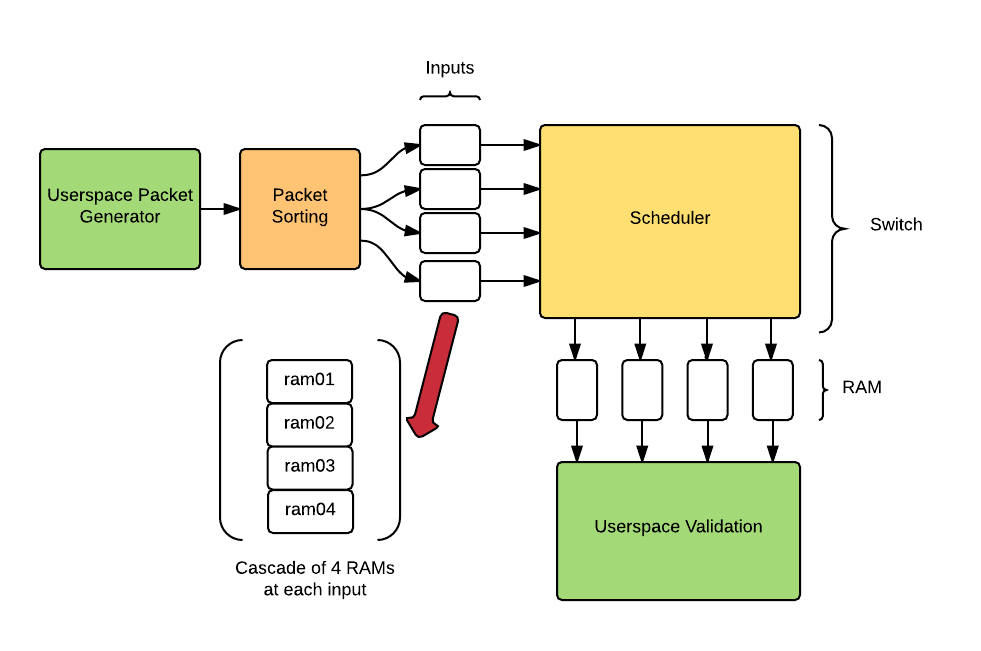
\includegraphics[width=0.9\textwidth]{block_diagram.png}
        \caption{Block diagram showing the overall functionality and flow of the system}
        \label{fig:block_diagram}
    \end{figure}
\newpage
The userspace packet generator is responsible for generating random packets each with:
\begin{itemize}
    \item 8 bits of header representing the destination port
    \item 8 bits storing the random seed that the data is generated based upon
    \item variable length data payload up to 64 bits
\end{itemize}
These packets are then sent to the packet sorting fabric on the FPGA which will decide which RAMs the packets will be sorted into based on the source port and the destination port. Each of the 4 inputs to the Scheduler has a cascade of 4 RAMs which identify which destination port the corresponding packet has to be routed to. The Scheduler then runs and proceeds to route the packets from the source RAMs into the corresponding destination port. The main aim of the scheduler is to maximise throughput by routing the most number of packets through the switch at every clock cycle. The RAMs located at the output then store these outputs. Each of the corresponding RAMs will only contain packets whose destination port corresponds to that specific output. The final step in the system is the Userspace Validation where the data stored in the memory locations of the output RAM will be retrieve and used to validate the integrity of the packets being sent through the switch.

\section{Hardware Section}\index{Hardware Section}
The hardware section of the entire system consists of the the following blocks as shown in Figure \ref{fig:hardware_section}. The hardware segment of the system is responsible for storing and routing the input packets into the correct destination output port. The hardware segment being implemented on the FPGA interfaces with the userspace software program using the master-slave architecture (CHECK). One thing to note is that the hardware architecture is not affected by length of the packet that needs to be routed, it will continuously route that same packet to the destination port until an 'end-of-packet' identifier has been reached. This is being transmitted as zeros of 32 bits in length.
    
    \begin{figure}[ht]
        \centering
        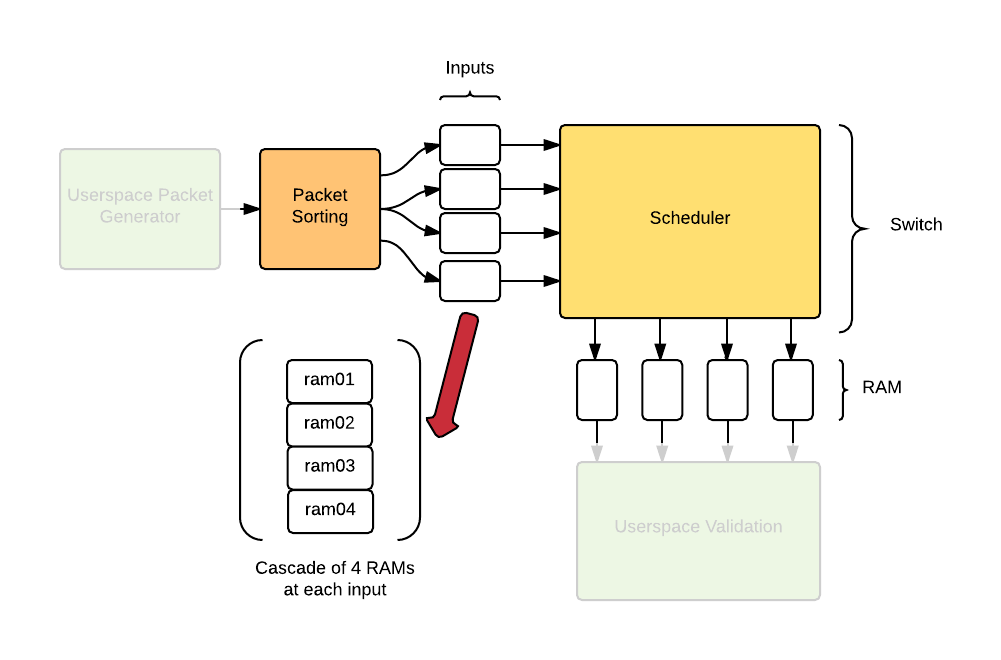
\includegraphics[width=0.7\textwidth]{hardware_section.png}
        \caption{Hardware segment of the system}
        \label{fig:hardware_section}
    \end{figure}
\subsection{Avalon Bus} The userspace talks to the FPGA using avalon bus. Userspace has access to various registers which are registered to to the device drivers which communicate through ioctl 32 read and write calls. In this project this is the only part that has not been evaluated on Verilator because the slides actually show the real scenario for the assert signals.Figure \ref{fig:avalonbus} and \ref{fig:avalon_write} shows the readdata and writedata transfer timing diagram that is used throughout in the project.
\begin{figure}[ht]
    \centering
    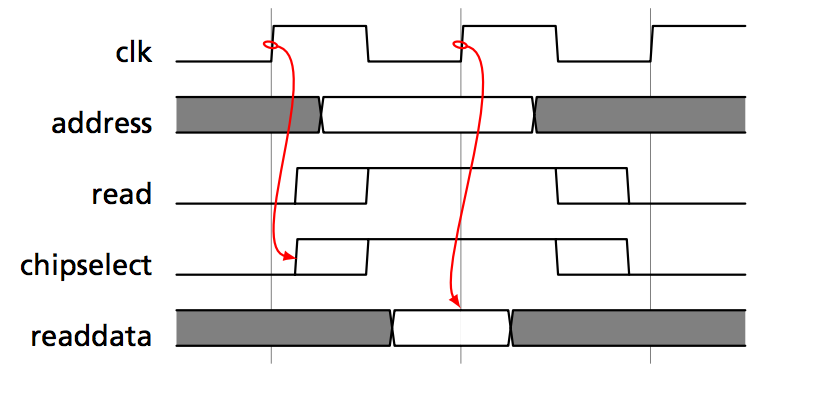
\includegraphics[width=0.7\textwidth]{avalonbus.png}
    \caption{Avalon Bus Read Signal}
    \label{fig:avalonbus}
\end{figure}
\begin{figure}[ht]
    \centering
    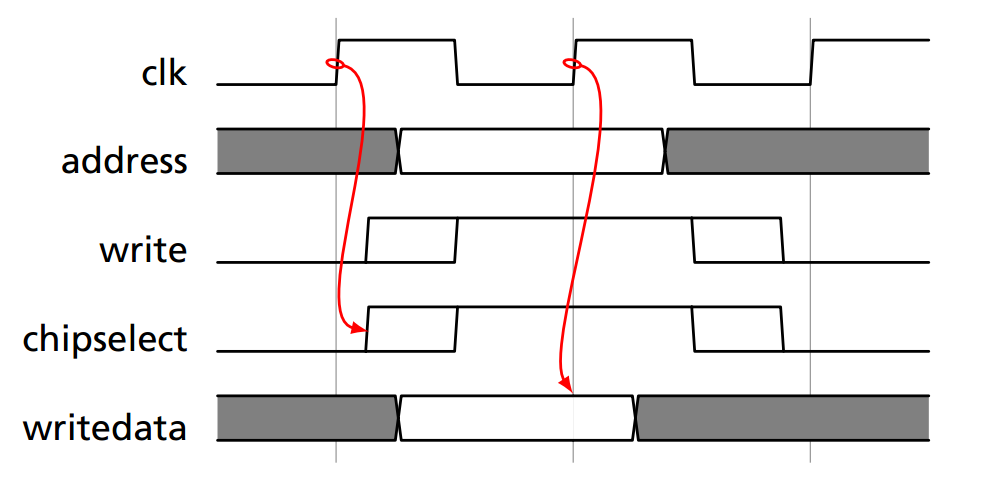
\includegraphics[width=0.7\textwidth]{avalon_write.png}
    \caption{Avalon Bus Read Signal}
    \label{fig:avalon_write}
\end{figure}
\section{Software Section}
The software segment of the system is responsible for generating the input packets and validating the output packets after it has been routed through the switch. This consists of the userspace packet generator and the userspace validator as shown in Figure \ref{fig:software_section} below. The userspace packet generator uses a random number generator to generate data payload of variable length of up to 64 bits in length. It also includes within that packet a header containing the destination port and the seed number that is used in that generation. This is done to ensure that at the validation side of the userspace, the software program can regenerate the given packet using that same seed number to verify the integrity of the packet. This will be explained in detail in a later section.
\begin{figure}[ht]
        \centering
        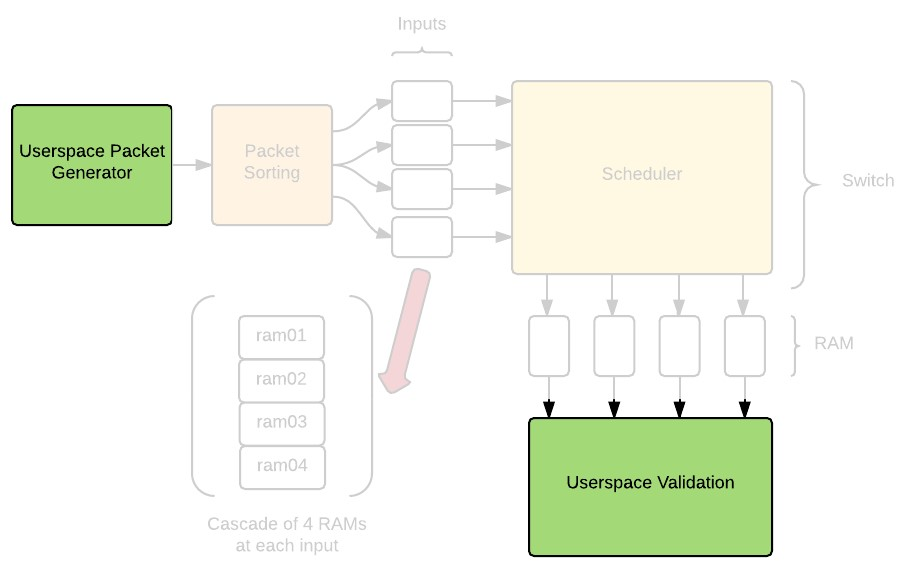
\includegraphics[width=0.7\textwidth]{software_section.jpg}
        \caption{Software segment of the system}
        \label{fig:software_section}
    \end{figure}


\chapterimage{simulation1.jpg}
\chapter{Simulation}

\section{Introduction}
The project depends heavily on simulations, so a robust test suite is created for the simulations. Out of the various compilers available for simulations Verilator was chosen for compiling the hardware code. An exhaustive test bench was created in C++ for interfacing with the compiled hardware code. Now it should be noted that the hardware code that is compiled is actually used in Quartus to compile it down on the hardware and therefore has some nuances and quirks. For example, Altera's compiler limits the number of iterations in the for loop to 255 which Verilator does not. Furthermore there are many such differences between the Verilator simulations and the actual hardware implementation and one should be careful while experimenting.

\section{Simulation Test Bench} Simulating Altera's IP core in Verilator was an integral as well as the most challenging part of the simulation. Since the project's progress contained different IP cores like Fifo , MUX and Ram. In the final design after many iterations several of these IP cores were removed/replaced but that would not have been possible without getting a deeper understanding of timing diagrams as well as the designed issues that needed to be resolved. 
\par SwitchON can simulate altera's IP core into the design using several caveats. For instance, the RAM module is defined in altera\_mf.v file in the eda simulation directly, but that file is not standard i.e it cannot be compiled by Verilator, hence several of the other components (~100k lines) have to be removed. Further more several helper functions needs to be added. Altera uses lots of tri state logic which does not simulate properly in Verilator, these can be removed but then care must be taken to add extra warning lints for, they cause the values to be used in block and no block. The veripool community is very helpful and some of the scripts they provided using Veripool-perl was instrumental in simulating the altsync RAMS. Again the idea was similar to converting the tri state logics to wire logics.

\subsection{Component Simulation} The test bench can compile each component separately as well as the full model suite. The ingenuity of such a modelling style allowed for amazing level of detailing that can be put to each module. This This allowed to optimize each clock cycle and made us achieve really high throughput through the scheduler. Each IP core has it's quirks and though it was frustrating when they didn't work the expected, it was really a nice learning experience.

\subsection{RAM Simulation} The simulation of altsync RAM was the most challenging part the project. First challenge was actually to find the library in which the module was defined. Running grep system wide did help to locate the module in the eda simulation directory of Quartus. But the RAM that altera uses has lots of tri state logics which prevent the data from coming to the output q port during verilator simulation, in Verilator's defense it did warn about those tri-state logics. Finally converting all such tri-states to wire leads to easy simulation of altsync RAM in verilator \footnote{There is a script by Todd Strader here \url{https://github.com/twosigma/verilator_support}. It can convert the tri-state logics directly to wire logic. Also, for a quick solution just convert the tri-state logics to wire and comment that section using appropriate verilator escape lint.}. Simulating results for the particular sections is shown in Evaluation.

\subsection{Conclusion} Verilator provides a really easy to use platform which is fast and actually simulates what goes into the hardware. The compilation time is actually nothing compared to Quartus and it provides a natural way to input any random signal into the model so that it can be tested to it's limit. Furthermore the output signals can be verified by just scripting the generated signals. It does have a steep learning curve but it's actually worth simulating.

\chapterimage{hardware.jpeg}
\chapter{Hardware Design}
\section{Interfacing with Software}
This is the front interface of the hardware. The packet data coming from the user space is received here. The main function of this module is to channel the packet data into appropriate RAMs. These RAMs are symbolic of the input ports of a network switch.

\subsection{Memory - RAM}
The Random Access Memory(RAM) modules are used in the system to simulate the input and output ports. These modules are implemented on the FPGA in the form of an embedded memory IP block supported by the Altera's Mega Wizard plugin in the Altera Quartus software.\\\\
A RAM is typically a type of computer data storage that allows data items stored into the memory module to be accessed quickly. It has typically much faster read and write times but is a form of volatile memory that loses its stored data when it loses power
\subsubsection{The Altera Embedded Memory IP Block}
The RAM modules that are implemented on the FPGA are of the form of a Simple dual-port RAM. This supports simultaneous one read and one write operations to different locations which is important in this system to minimise the number of clock cycles required to access data from the RAMs. Figure \ref{fig:RAM_input} below shows the inputs and outputs that are configured for the RAM module. It takes in the input clock from the overall clock of the system, has a word length of 32 bits and a storage space of 4096 words. These are controlled by the input signals rden(read enable) and wren(write enable).\\\\
Figure \ref{fig:ram} shows the timing diagram of the Altera RAM module.
\begin{figure}[ht]
        \centering
        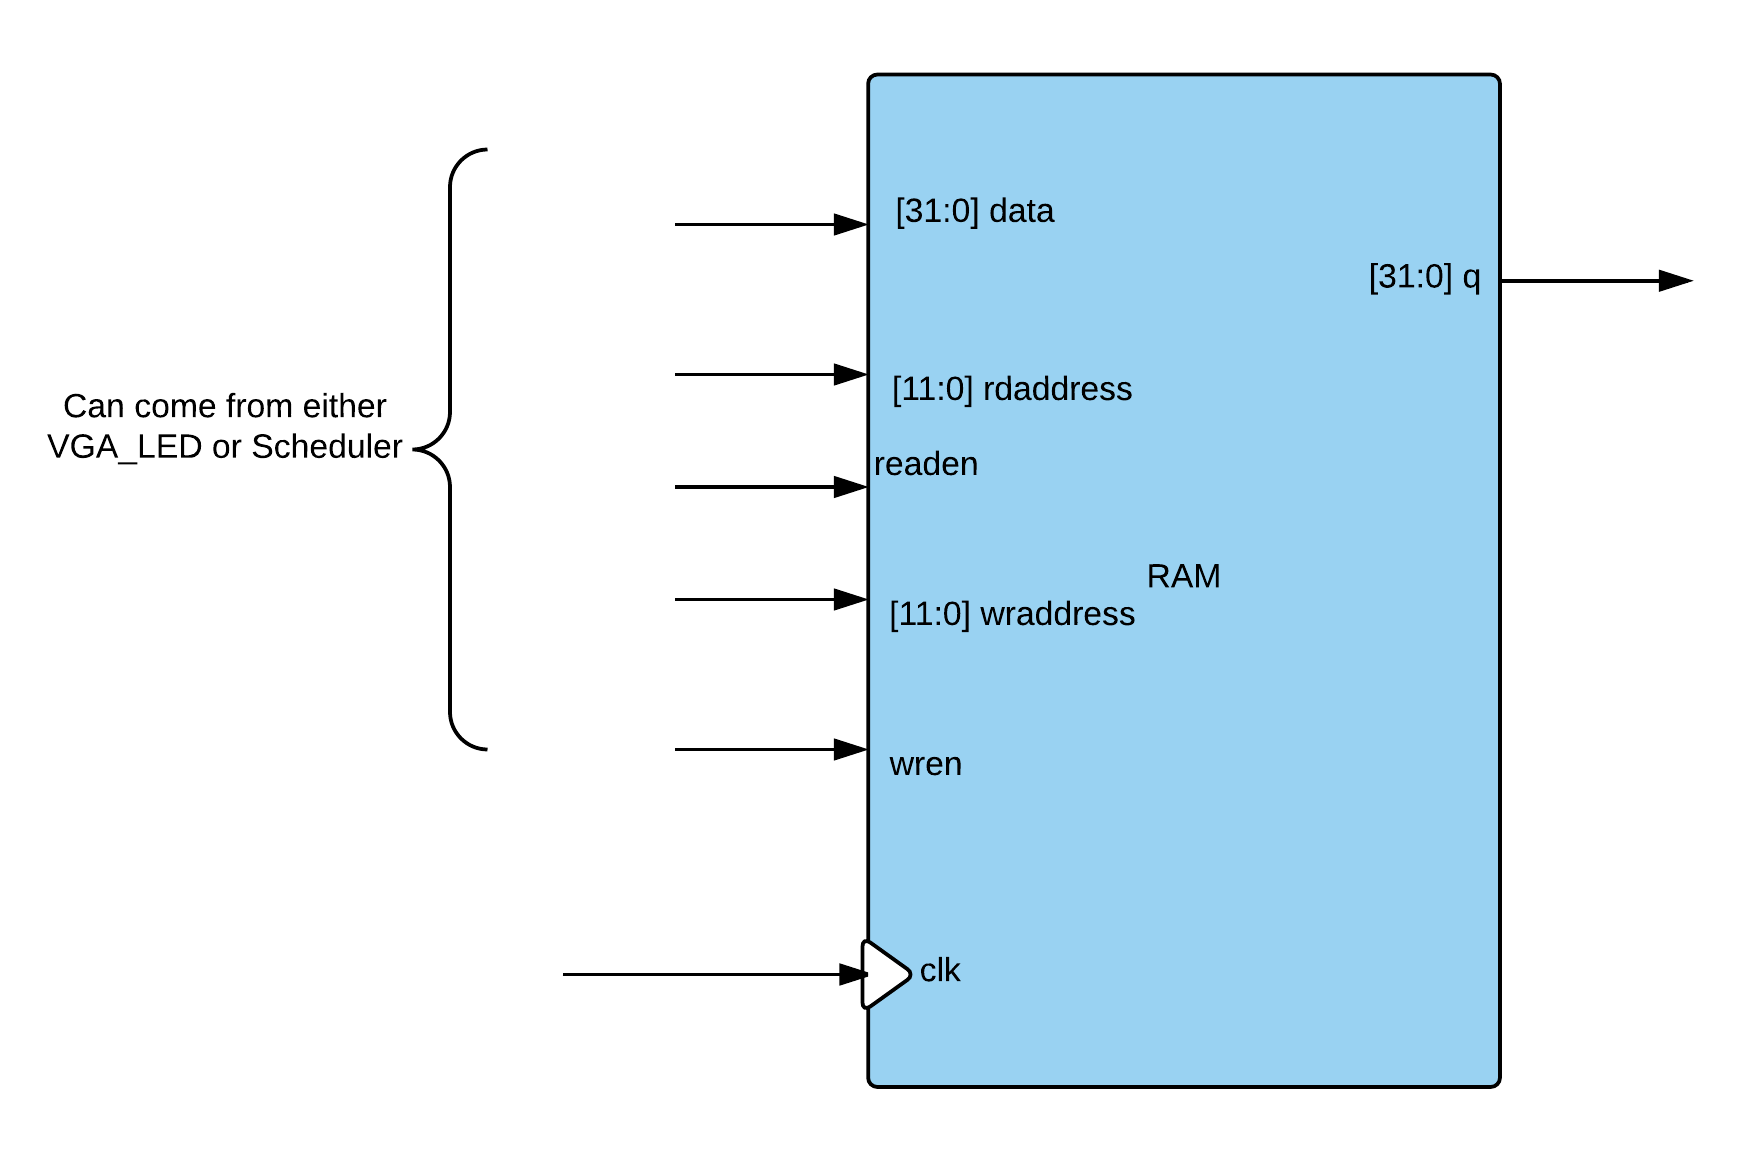
\includegraphics[width=0.8\textwidth]{ramblock.png}
        \caption{Snippet of code showing the inputs and outputs attached to the RAM module}
        \label{fig:RAM_input}
    \end{figure}
    \begin{figure}[ht]
        \centering
        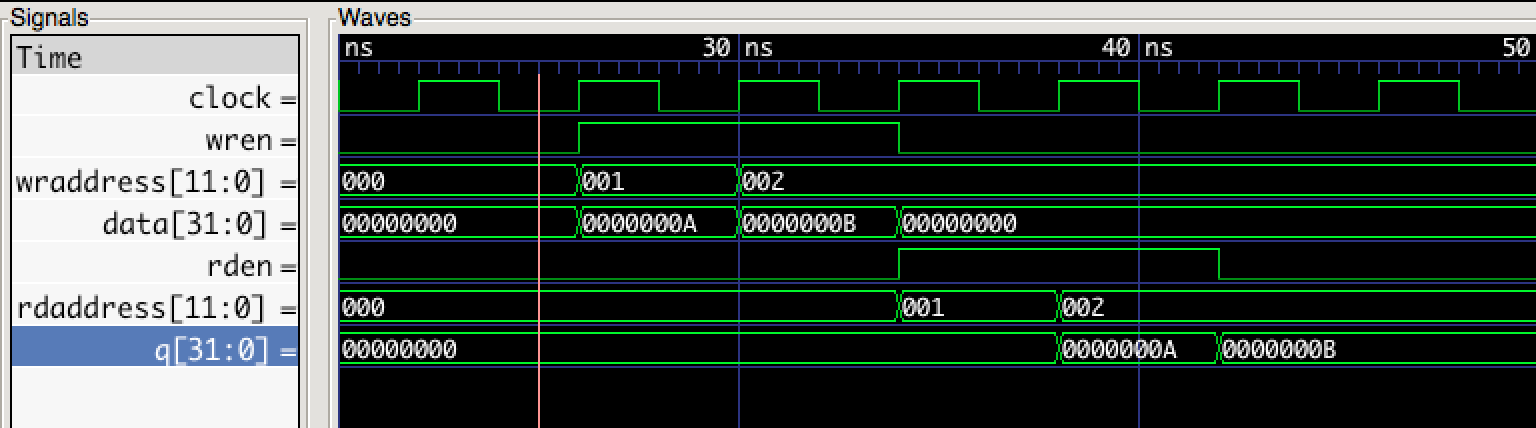
\includegraphics[width=\textwidth]{ram.png}
        \caption{Timing diagram of the read and write operations of the RAM}
        \label{fig:ram}
    \end{figure}

\section{Network Fabric}
A network switching fabric is the hardware topology of the network that is laid out and is responsible for transporting the input packet to its respective output port. The network fabric being employed in this project is the crossbar architecture. The crossbar architecture is basically a network topology that is in the form of a matrix as shown in Figure \ref{fig:crossbar_illustration} below: 
    \begin{figure}[ht]
        \centering
        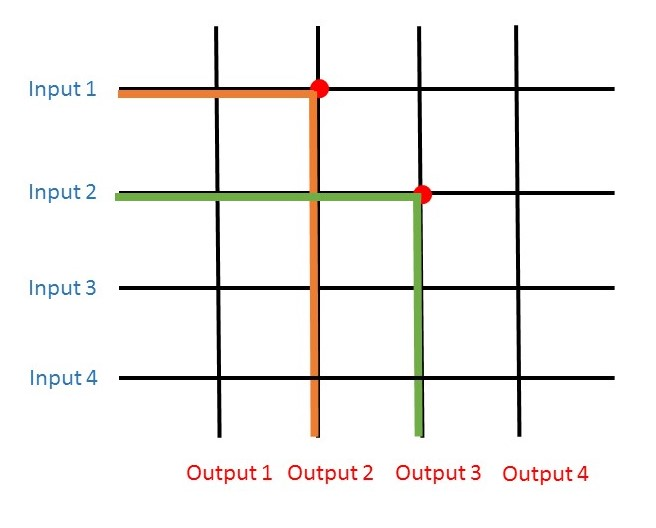
\includegraphics[width=0.65\textwidth]{Crossbar_Architecture.jpg}
        \caption{Illustration of the Crossbar Architecture that will be responsible for the network switching fabric}
        \label{fig:crossbar_illustration}
    \end{figure}

\subsection{Crossbar Switch Model}
In this project, a single layer 4$\times$4 topology with 4 inputs and 4 outputs is utilised. The Figure \ref{fig:crossbar_illustration} above illustrates how every input is being connected to every output by the intersections of the matrix, termed crosspoints. The implementation of the crossbar switch model is done on the FPGA. Each input to output connection is completely independent of each other and can therefore support simultaneous communications, except in the case when two ports wish to use the same output port. 

\subsubsection{How the Crossbar Switch Works}
The crossbar switch architecture works in a similar way to that of active addressing in an LED(Light emitting diode) matrix. The inputs are connected to every output by lines that can be turned on and off depending on the destination of the source packet. For example in Figure \ref{fig:crossbar_illustration}, the orange line shows how the input 1 is able to send a packet through the network fabric to output 2 by turning on it's horizontal line and the vertical line that corresponds to output 2. As mentioned earlier, the lines are independent of one another and therefore in a single time slot, both input 1 and input 2 can send packets to outputs 2 and 3 respectively without colliding. Theoretically and in some cases practically it is possible to get \texttt{n}\footnote{where n is number of output ports,in this case 4} number of packets in the output.

\subsubsection{Implementation in the system}
\begin{figure}[ht]
    \centering
    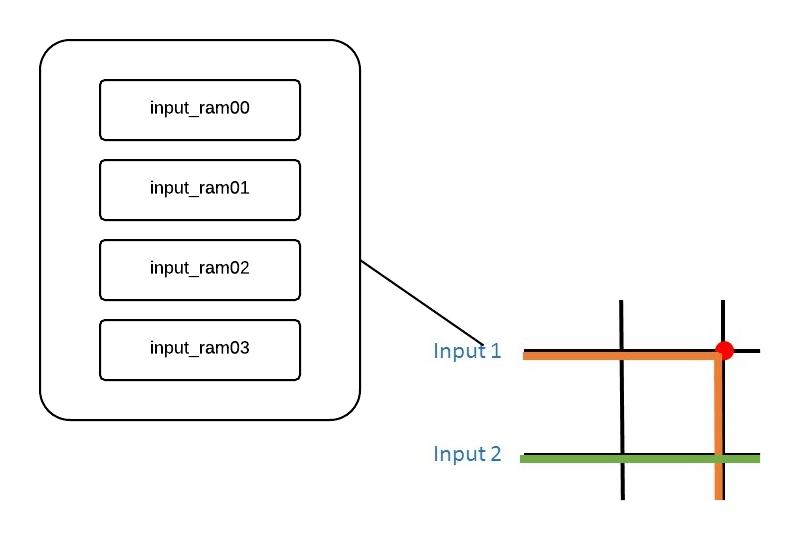
\includegraphics[width=0.8\textwidth]{input_blowup.png}
    \caption{An exploded view of a single input port to the network fabric}
    \label{fig:input_blowup}
\end{figure}
In our implementation, 16 RAM modules are used at the input port of the network fabric. This means that each input port of the network fabric has exactly 4 RAMs, one for each output port. They have the above mentioned capacity and word length. This is as shown in Figure \ref{fig:input_blowup}. 
The functionality of these input rams are to store the packets distributed according to their output ports. When the scheduling algorithm runs and selects the packet to be routed through the network fabric to the output ports, the stored packets are accessed and removed from the input RAMs and routed through. The exact same RAMs are utilised in the output port for storage of the routed packets. 

\section{Scheduling Algorithm}
The Scheduling algorithm is at the core of the network switch. The scheduler makes all the decisions regarding the routing of the packets. It looks at the incoming packets and based on the header decides the output port of the packet and routes the content accordingly.\\\\
The first preference to the scheduler is always correctness; to make sure none of the packets are lost. The priority is that all the information is transferred as required. Then comes the efficiency. How fast the scheduler can route the data on the input ports utilizing the least number of clock cycles. The scheduling algorithm for our project was also developed in similar two stages.\\\\
Another important thing to add is that the hardware code is agnostic to the size of the packet. It marks the start of a packet with a header, containing the port information, followed by unknown number of 32 bit words followed by a 32-bit zero value to mark the end of packet. Once the zero value is encountered, the Scheduler understands that the packet has ended and prepares itself for the next packet.\\\\
One performance constraint with both the designs is the RAMs that have been used to simulate the input and output ports. 3 clock cycles are required to analyze and transfer each 32 segment of the data. This is required by the RAM. It takes one clock cycle to increase the address and another for the output to appear. While working with two clock cycles also, sometimes the data would appear late resulting in consistent errors. Another clock cycle has to be spared to make sure that the data is stabilized. So the speeds that are achieved can be scaled by an appropriate factor considering the real world scenario.\\\\
We here discuss the Scheduler algorithm. The initial design focuses only on correctness while the second one tries to improve the performance with some additional hardware logic. Both designs will be discussed below.
\subsection{Single Input Queue Scheduler}
The initial design of the scheduler was a simple crossbar switch. The scheduler looks at the head of the packets on different ports, and simply routes the data according to that information. In case of collision, the data is transferred one by one, holding the data at one of the ports while the other one is transferred and then transferring the data from the next port.\\\\
The preference in case of a collision is always given to the lower numbered port. What this means is that if there are two packets at ports 1 and 2 both waiting to go to the output port 2, the preference will always be given to the packet at port 1. The upside to this approach is that it is very simple to implement. The downside being that if the next packet on port 1 also has to go to port 2, it will still precede the packet on port 2. This can lead to starvation and theoretically the port 2 packet may never flow through, if all the packets on port 1 are to destined to port 2.\\\\
The way the scheduler achieves this is by storing state of different input ports. One variable per port to store the destination port of the current packet coming in through the input port. Another variable is used to indicate the End-of-packet signal which meant the scheduler had to to refresh its transfer information in the next cycle. \\

\subsubsection{PPS Architecture}
\begin{figure}[ht]
    \centering
    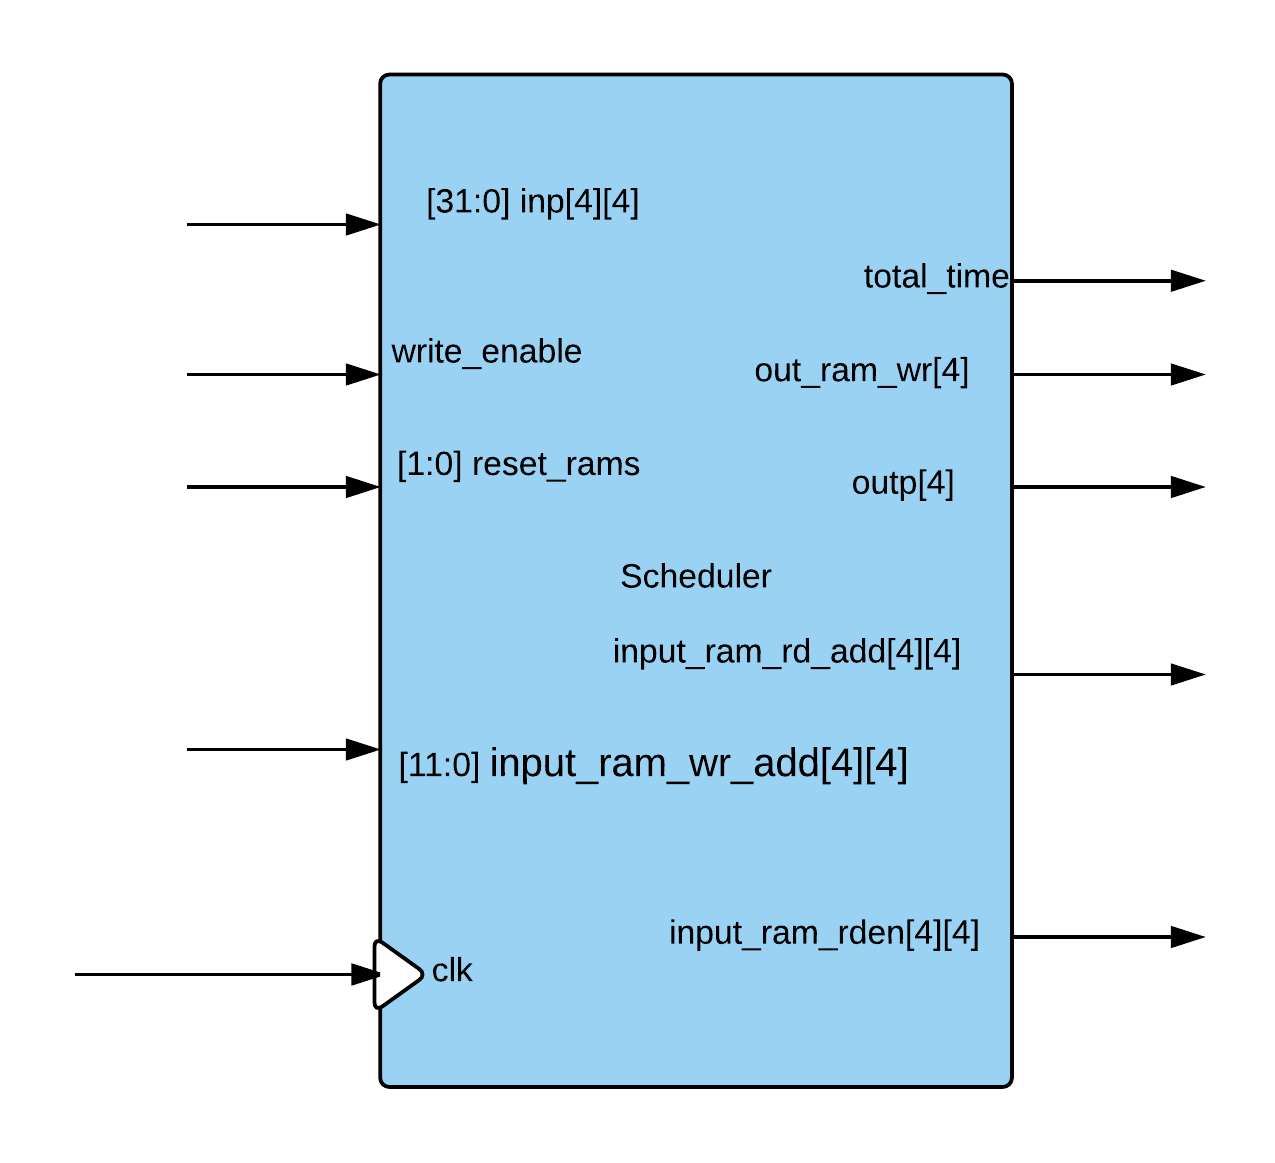
\includegraphics[width=0.8\textwidth]{schedulerblock.png}
    \caption{Block Diagram of the Scheduler}
    \label{fig:scheduler_block}
\end{figure}

\begin{figure}[ht]
    \centering
    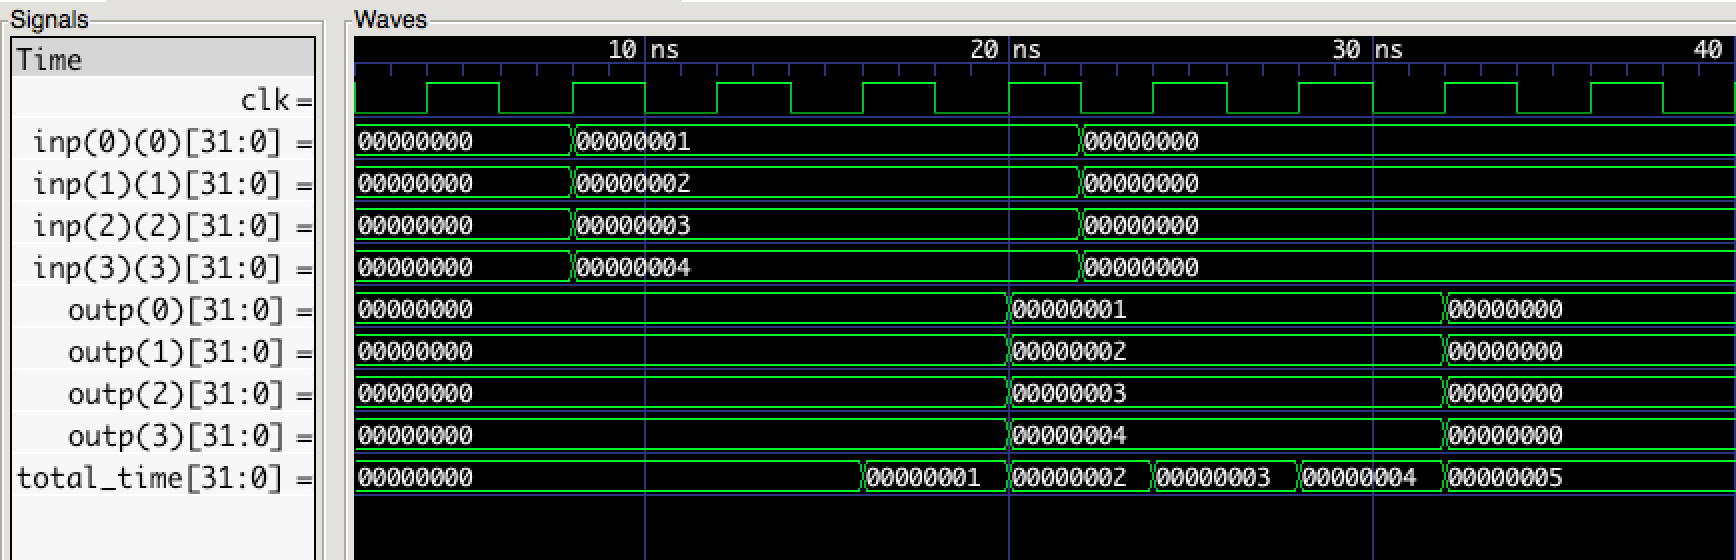
\includegraphics[width=\textwidth]{scheduler1.png}
    \caption{Scheduler timing diagram showing packets to different output ports}
    \label{fig:scheduler1}
\end{figure}

\begin{figure}[ht]
    \centering
    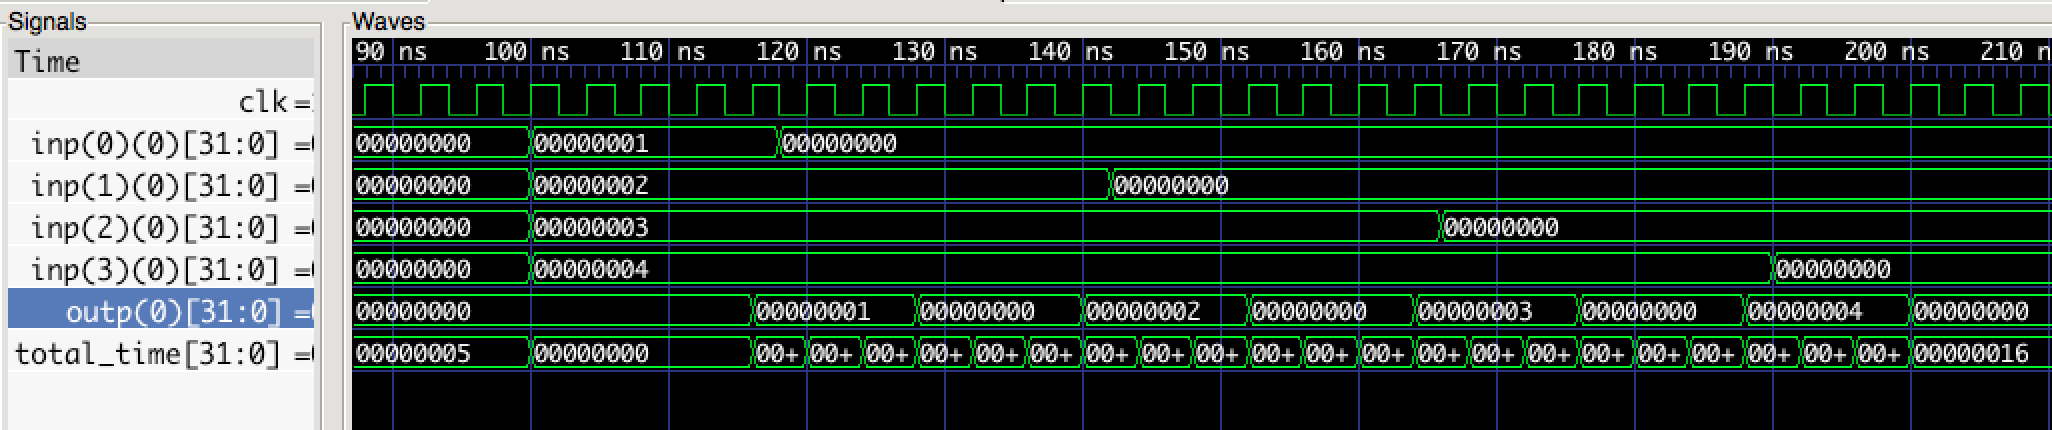
\includegraphics[width=\textwidth]{scheduler3.png}
    \caption{Scheduler timing diagram showing packets to the same output port}
    \label{fig:scheduler2}
\end{figure}
In the second part of the project an attempt to optimize the performance by adding hardware complexity is discussed. Instead of using one RAM per port, four (the number of output ports) such RAMs are used per port. For the user space, the packets are still being sent to the four input ports instead of sixteen. However, a layer inside the hardware divides these packets based on their output destination.\\\\
Figure \ref{fig:scheduler_block} show how the Scheduler looks like. the inp[4][4] signals are the input signals from the rams. input\_ram\_rd\_add signals control the address of the ram from which data is being read. The outp[4] signals are the output signals which contain the packets on their destination port and out\_ram\_wr are to control writes to the output RAMs.\\\\
The way it helps is that segregation of packets based on their destination ports greatly improves timing efficiency. A packet meant for the output port two does not have to wait behind another packet meant for output port one. It eliminates the time where one or more output ports has to wait lying empty because none of those packets were at the front of the queue on their respective input ports.\\\\
This approach optimizes for different ports but still faces the starvation problem faced by the initial design because here also the preference always goes to the packet on the port one. It still performs better because packets for other ports does not have to be stuck because the front packet cannot pass through.\\\\
Figure \ref{fig:scheduler1} and \ref{fig:scheduler2} give the timing diagrams of the scheduler implemented. While Figure \ref{fig:scheduler1} shows the situation where packets to different output ports appear on the input ports, the Figure \ref{fig:scheduler2} shows the case, where all packets are meant for the same output port.

\subsection{Performance Comparison}
\begin{figure}[ht]
    \centering
    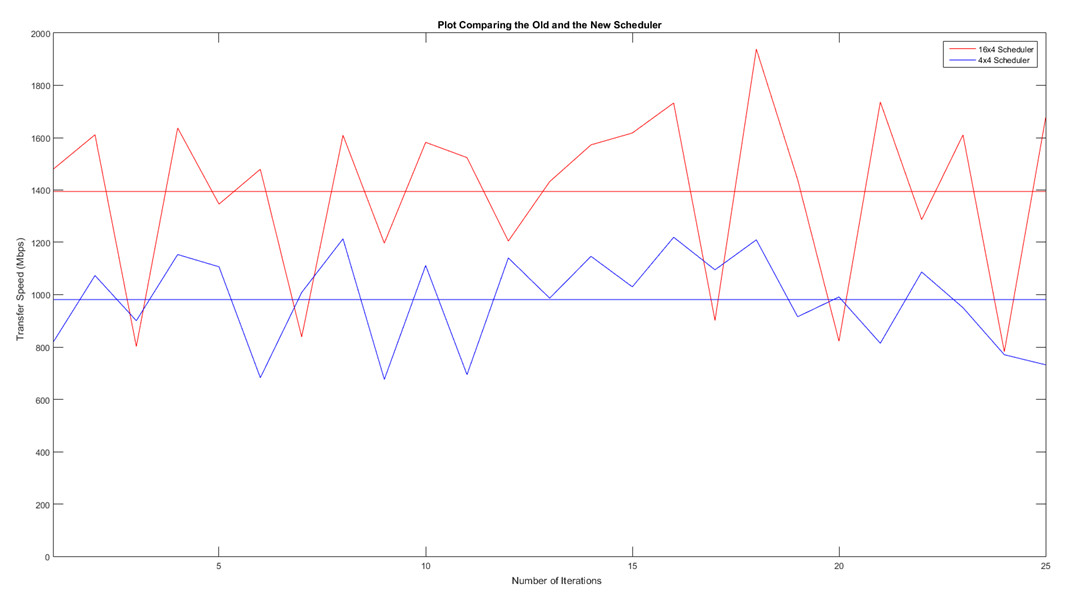
\includegraphics[width=\textwidth]{Comparison_scheduler.png}
    \caption{Comparison plot of the performance achieved with the two Scheduler algorithm}
    \label{fig:comparison}
\end{figure}
A comparison of performance between both Scheduling algorithm is done to investigate the differences. Random test runs of 100 packets of lengths ranging from 4 to 64 uniformly spread across the source ports but randomly across the destination ports. Figure \ref{fig:comparison} shows the relative average speeds achieved by using the two different Schedulers. The performance statistics for the initial design is shown in red while blue highlights the performance of the optimized scheduler.\\\\
It is clearly visible that the optimized algorithm shows higher performance both in terms of average as well as the most optimal performance. The performance of the initial design is lower which is consistent with the expectation from the algorithm. While it is easy to see that the average performance is higher, the worst case scenario for both cases occurs when all the packets are scheduled to the same output port. The calculation for such a case is as follows:
Since, 32-bits of data is transferred every three clock cycles:
$$ Speed = \dfrac{32}{3} bits/cycle$$
$$ Speed = \dfrac{32}{3\times20\times10^{-9}}$$
$$ Speed = 0.533\times10^{9}$$
$$ Speed = 508.626 \hspace{1mm} Mb/s $$\\
This comes out to be consistent with the data presented in the test runs. If the test bench is modified to ensure that all packets are sent to the same output port, the transfer speed matches the above mentioned speed up to three decimal places.\\\\
This also gives a logical explanation for the wider variance seen in the optimized algorithm graph as compared to the initial one. Seen the spectrum for the optimized algorithm is higher with a higher average, the variation and the peaks are also higher.
\subsection{The whole suite}
Figure \ref{fig:vgablock} shows the block diagram of the entire suite and its interaction signals with the avalon slave bus. Figure \ref{fig:vga1} and \ref{fig:vga2} show the timing diagrams of the flow of packets to and from the user space. It can be seen that the sanctity of the packets is maintained in its movement through the system.
\begin{figure}[ht]
    \centering
    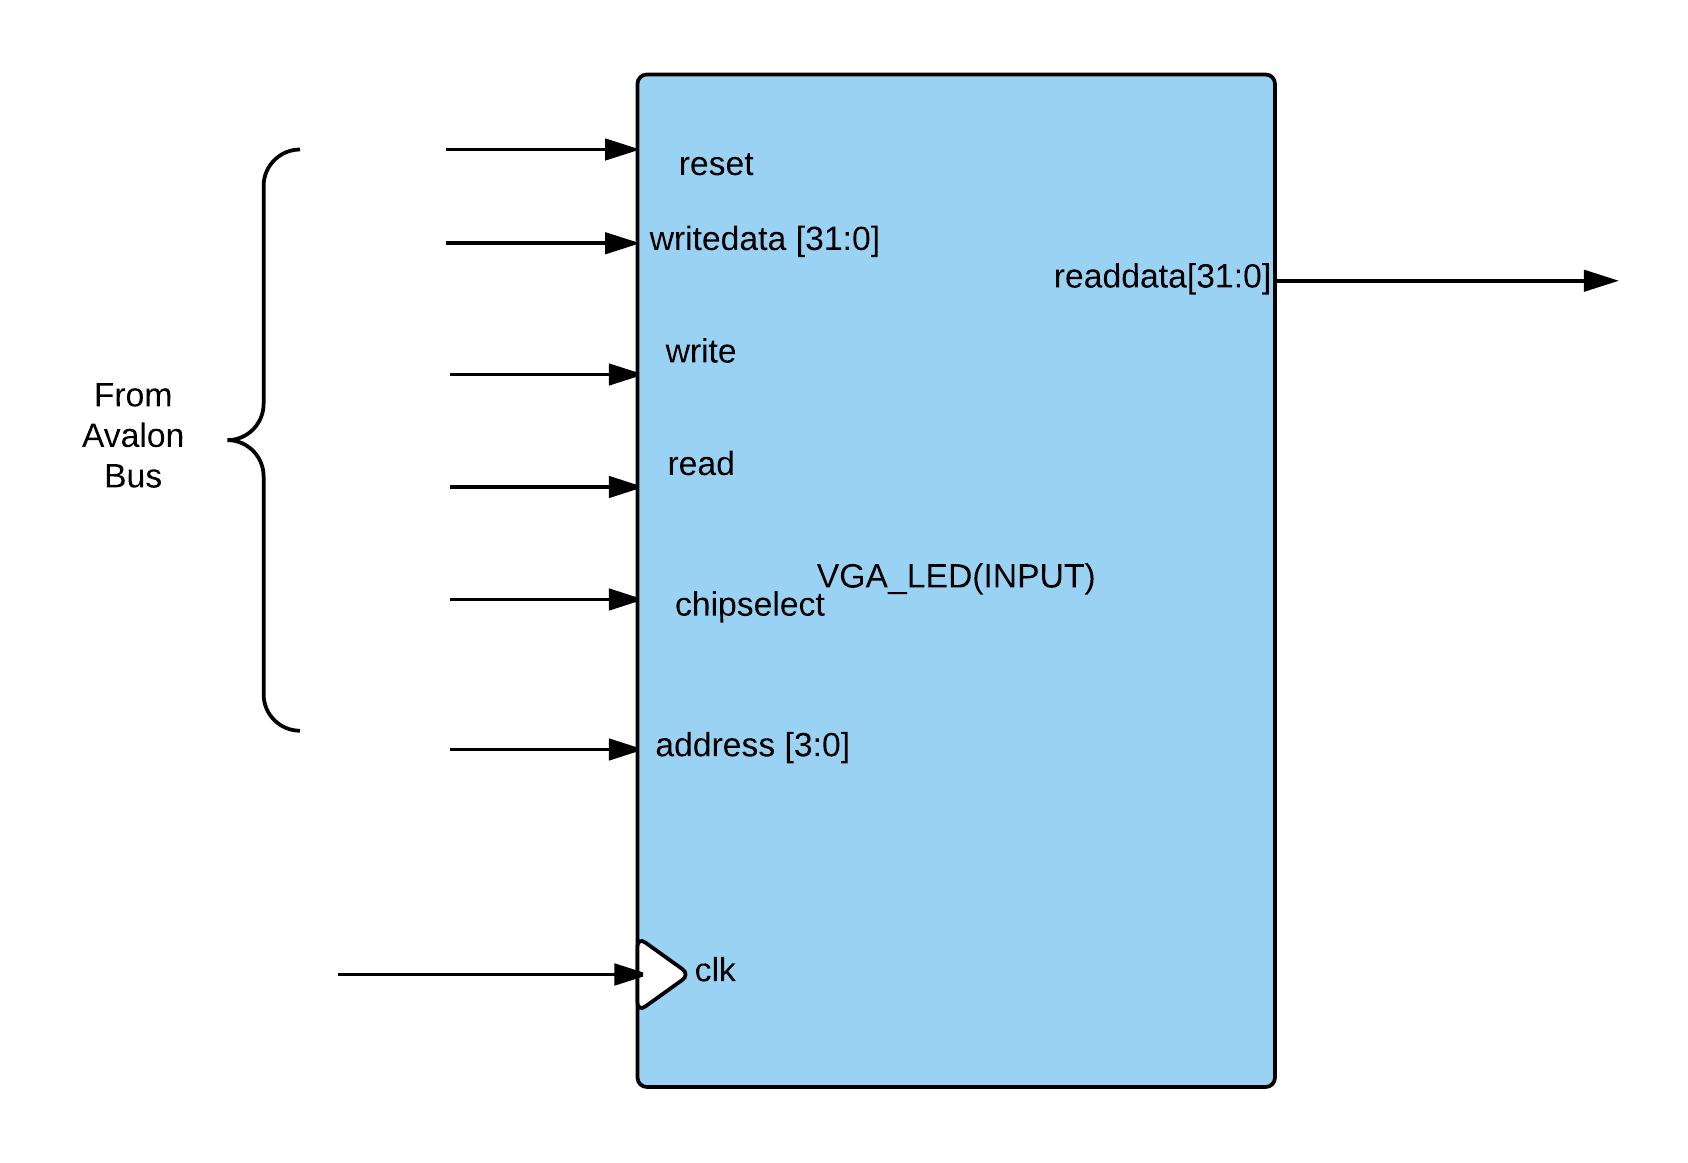
\includegraphics[width=\textwidth]{vgaledblock.png}
    \caption{Flow of packet from the user space}
    \label{fig:vgablock}
\end{figure}
\begin{figure}[ht]
    \centering
    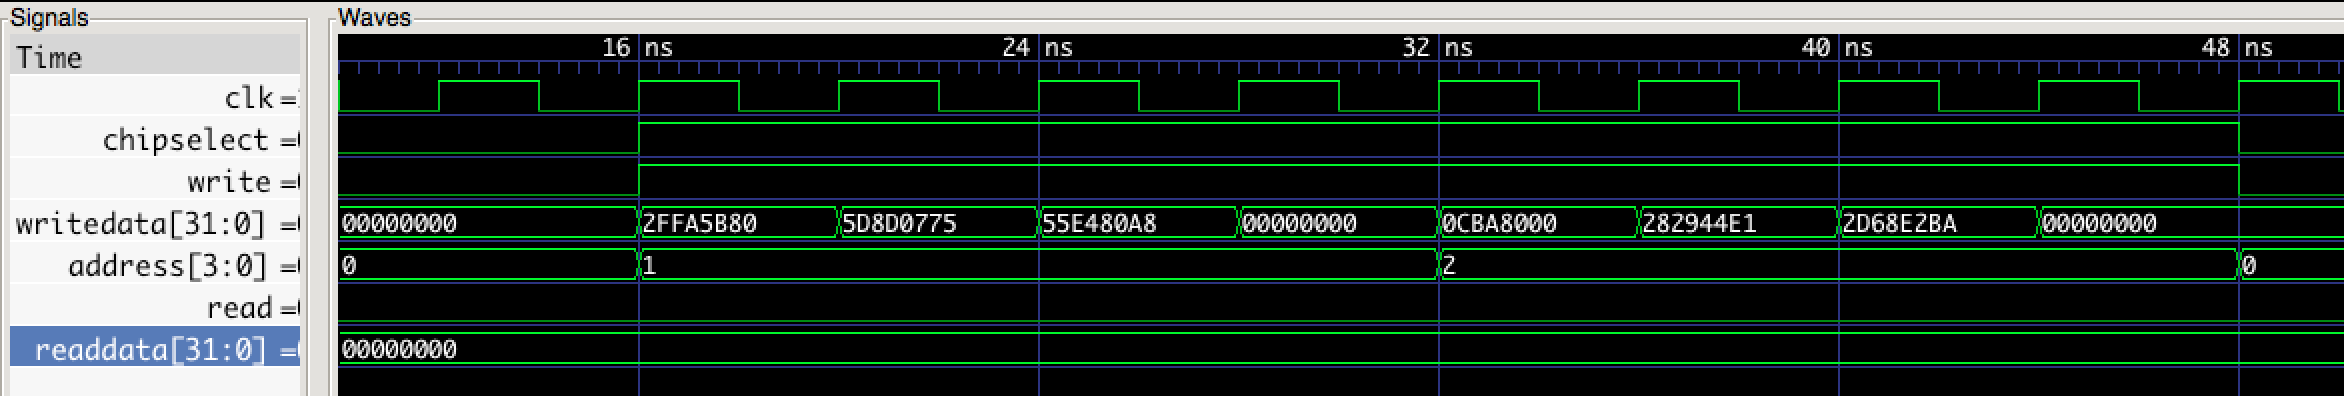
\includegraphics[width=\textwidth]{vga1.png}
    \caption{Flow of packet from the user space}
    \label{fig:vga1}
\end{figure}
\begin{figure}[ht]
    \centering
    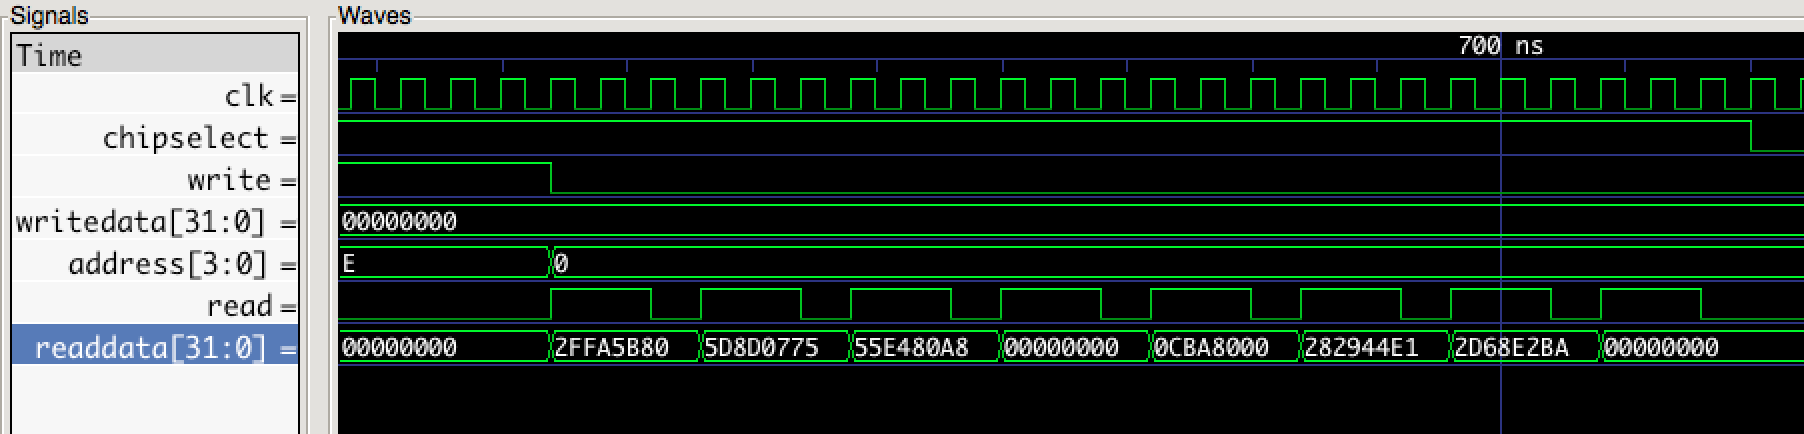
\includegraphics[width=\textwidth]{vga2.png}
    \caption{Flow of packet to the user space}
    \label{fig:vga2}
\end{figure}

%----------------------------------------------------------------------------------------
%	CHAPTER 3 SOFTWARE
%----------------------------------------------------------------------------------------
\chapterimage{software.png}
\chapter{Software}
The software side talks to the Hardware using the ioctl32 calls. It also generates the packets which are to be routed through the Switch. Furthermore it reads back from the Output RAMS and locally generates the packet and verifies it, if all packets pass the verification it then calculates the throughput through the Switch for that iteration.
\section{Implementation details }\index{Software details}
The userspace consists of:-
\begin{itemize}
    \item Packet Generator: It generates seeded random number of packets upto NUM\_PACKETS(defined in packetgen.h file). 
    \item Validator: After packet transfer is complete validator runs over the contents of each RAM verifying for consistency in terms of content and port matching.
\end{itemize}
\subsection{Packet Generator}
Packet Generator consists of packetgen.c and packetgen.h. The entry point to these modules is through main.c. Based on the seeded input value it generates a 32 bit random number of which each 8 bits except the first 2 MSB bits have their own \texttt{minimum requirements} which are again defined in packetgen.h header file.
\par\vspace{\baselineskip}
Once the packet generator has sent all the packets using the ioctl32 calls before shutting itself off, it sends the WRITE\_ENABLE\_SCHEDULER and READ\_ENABLE opcodes to the module which kicks in the Scheduler.
\begin{table}[ht!]
\begin{center}
    \begin{tabular}{| l | l |}
    \hline
    Last Bits & Output Port \\ \hline
    0000 0000 & Port 0 \\ \hline
    0000 0001 & Port 1 \\ \hline
    0000 0010 & Port 2 \\ \hline
    0000 0011 & Port 3\\ \hline
    \end{tabular}
    \caption{I/O Mapping from RAM}
	\label{table:io_mapping}
\end{center}
\end{table}
\subsection{Validator}
After the FPGA processing when the packets are routed to their appropriate output ports (modeled by memory locations) the validator runs and checks that the packets should be stored on correct memory locations. As discussed above, the generated packet consists of random sequence of bits with the last two bits representing the destination port. The validator makes sure that this values matches the memory space in which the packet is stored and reports any errors encountered.
\par\vspace{\baselineskip}
The validator validates the packets which are received from the output RAMS. Now using the stored seed, the validator seeds itself to stored seed and then starts generating the packets locally. Now each octal of the received packet part is compared against the locally generated octal, if match happens it that part of the packet is marked OK and the validator moves to check other packet. Now should a packet not match the generated seed, error is thrown and the program exits. For the simulation scenario,it is ensured that none of the packets are dropped and none of the packets are wrongly stored.

After all the validation passes, the validator sends an OP-Code to the FPGA which then returns the total\_clock\_cycles it took to transmit that data. Using this information the throughput of the Switch for that particular iteration can be calculated. It has been observed that both in case of PPS and Single Input Architecture the throughput fairly remains constant with a small swing along the average $\pm$ 200 Mbits/s, which is fair in terms of packets that are being sent. In other words since the packets are being generated randomly it might so happen that the generation might be skewed towards a particular output port, which leads to number of cycles being increased as packets are now queued thus leading to more time for transfer. This issue will be fairly common in both the architecture because all the packets can now go to only one part,so in each clock cycle a single packet will be transferred, in other words packet transfer would be linear.
%----------------------------------------------------------------------------------------
%	CHAPTER 4 Metrics
%----------------------------------------------------------------------------------------
\chapterimage{metrics.png}

\chapter{Evaluation}

\section{FPGA Switch Performance}\index{FPGA Switch Performance}
Having implemented and tested the functionality of the FPGA switch, the next step would be to evaluate the performance of the switch and how it performs under various types of load. 

\begin{figure}[ht]
    \centering
    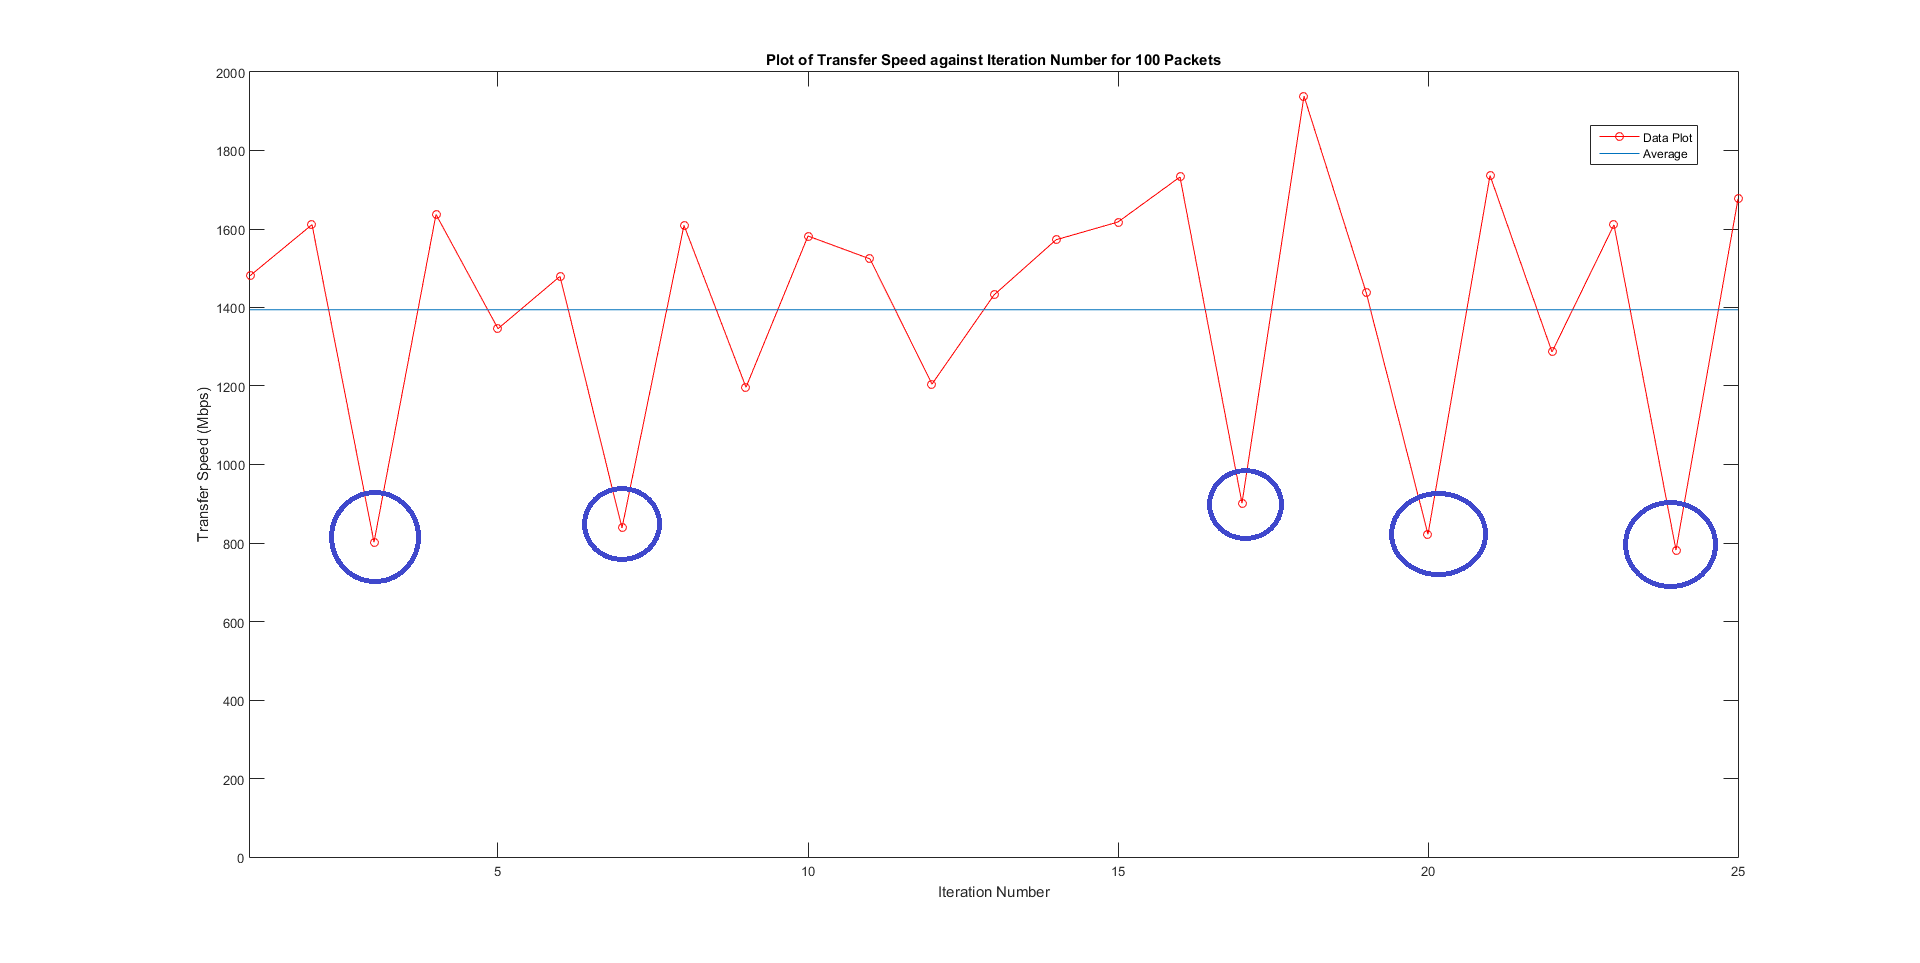
\includegraphics[width=1\textwidth]{speed_plot.png}
    \caption{Plot showing the data transfer speed over 25 iterations}
    \label{fig:speed_plot}
\end{figure}
The first test is to measure and find the average speed of data transfer that the switch is capable of achieving. This is shown in Figure \ref{fig:speed_plot} above. It can be seen that there are massive fluctuations in the data plot, there are however some points to note which are circled in blue. These points are outliers in the data plot that occurs whenever there is a concentrated number of packets that are sent to a specific port. Due to the random distribution of packets that are sent to each destination port, there will be a case where for example 50 of the 100 packets generated are destined to output port 3. Such a data point will then result in an outlier where the data transfer speed is severely crippled because a higher number of clock cycles are required to process that concentration of packets destined for a single output port. The average transfer rate of the switch including these outliers still remains at an impressive speed of approximately 1400 Megabits/second (Mbps)
 
\begin{figure}[ht]
    \centering
    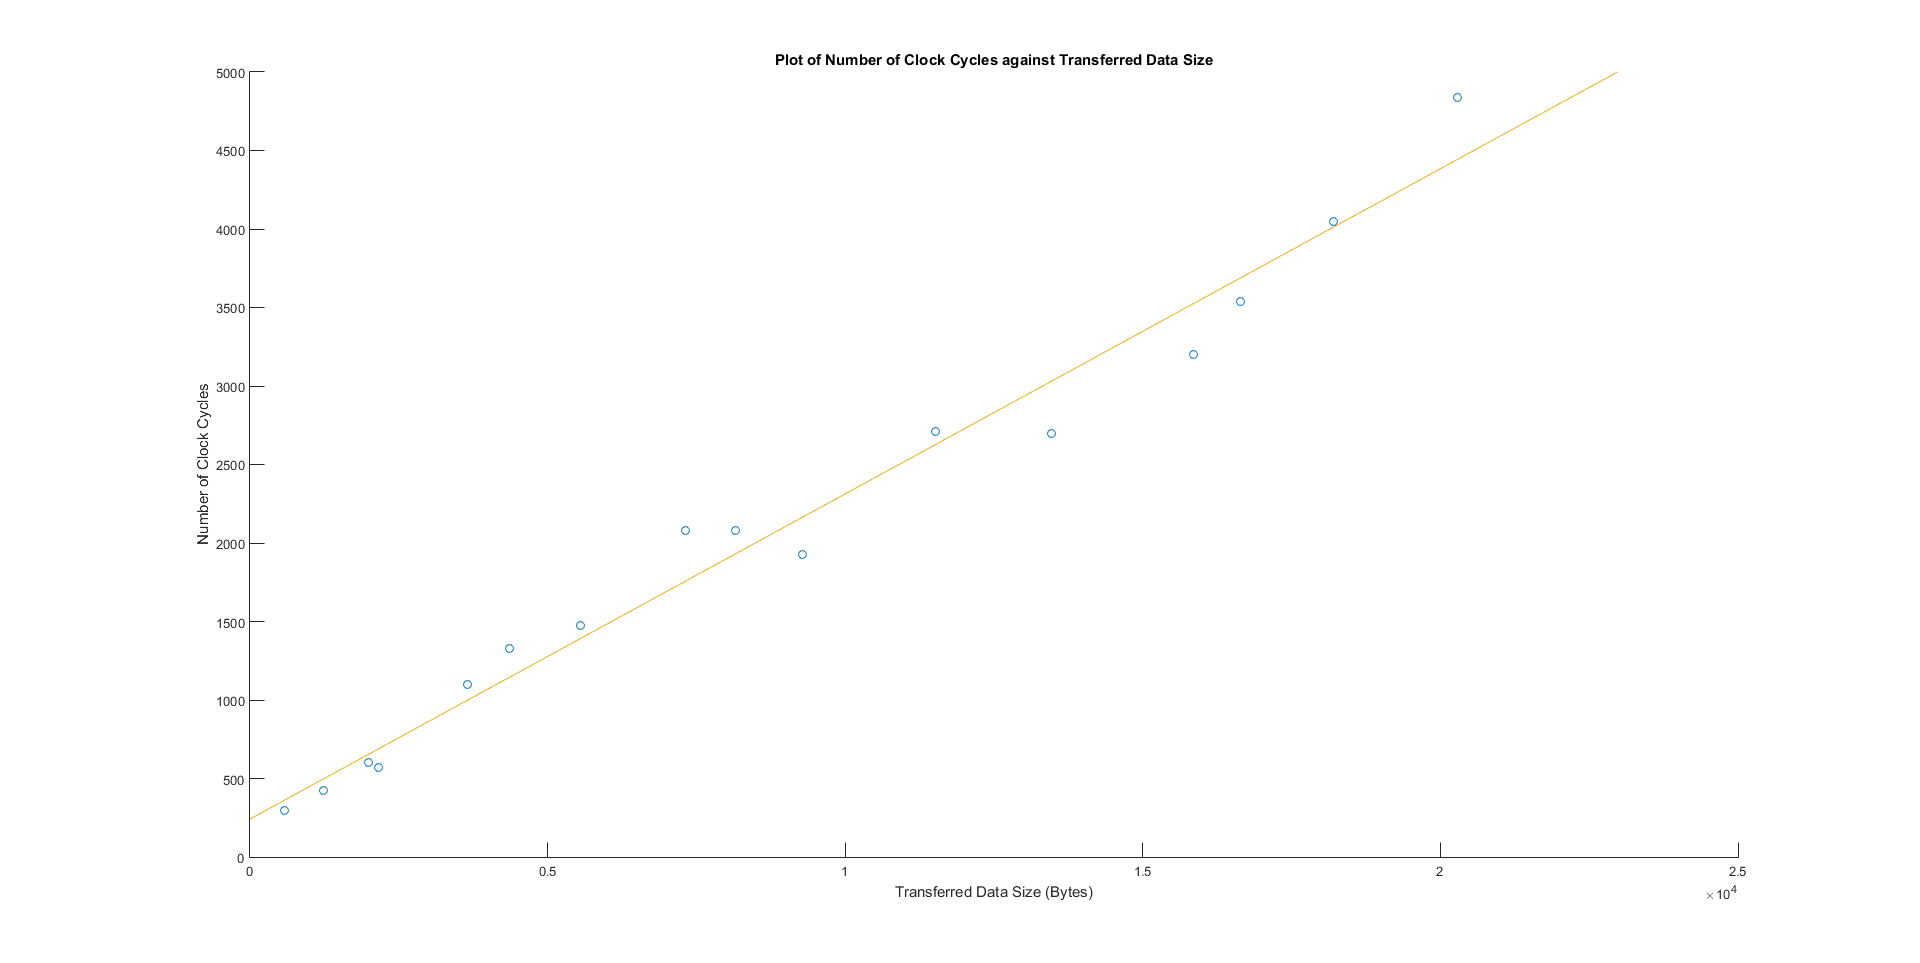
\includegraphics[width=1\textwidth]{clockcycle_plot.png}
    \caption{Plot showing the the number of clock cycles needed to process a given data size}
    \label{fig:clock_cycle}
\end{figure}

The second test involves incrementing the total transferable data size to investigate how the number of clock cycles required to complete the routing changes. It can be seen from the Figure \ref{fig:clock_cycle} that the number of clock cycles required increments linearly with increasing data sizes. The gradient of the slope gives the data transfer speed at that given point, seeing as how the graphs proves to be a linear plot, it is safe to say that the transfer speed of the switch remains constant regardless of the transferable data size. This means that under heavy data loads, the switch will still be able to perform at its maximum capacity. 


\chapterimage{thatsall.png}

\chapter{Conclusion}

Using the simulated Switch implemented in hardware, it can be concluded that for all real cases in which the packet arrival can be Poisson, PPS architecture would be really helpful because then Head of line blocking can be avoided and throughput would increase as can be seen from the results. Furthermore it's futile to expect that the throughput would increase in the order of the input ports because of the distribution in which the packets arrive. Though this can be avoided using fixed input ports for a particular packet sizes, but is not entirely avoidable.

\par 
\section{Lessons Learnt}

Throughout the course of the project, there are a few lessons to be learnt:

\begin{itemize}
    \item Hardware is hard. Like seriously programming hardware is very different from working on just purely software. In software, logic take precedence where a good logic will mean an efficient and perfectly functioning piece of code. This differs greatly in hardware where logic has to be perfect but also timing of every hardware module must be taken into consideration due to data stability reasons,few modules might be slow in giving out the data so everything cannot work as per the designed clock cycles.
    \item Simulating what hardware does in software that produces timing diagrams is the best way to debug hardware issues. Timing diagrams while tedious and time-consuming to do and set up, provide an insight into what the hardware is actually doing, saving you time in the end.
    \item While simulations provide insight, it may not be truly representative of what actually goes on in hardware. More often than not, the simulations hold true. But every once in awhile, it goes way off tangent so always check what the actual hardware is telling you. For example there were cases in which Verilator would actually simulate the altsync ram, but there would be no output on the q port. Furthermore Quartus limits the number of iterations to 255 in a for loop, but since verialtor is platform agnostic it synthesizes the code,hence there might be a case in which the logic would work in Simulation only to fail in hardware.
    \item Hardware documentation is not as robust as those that you will find on open sourced stuff such as python libraries. Simulating and creating test benches early and often is a nice way to debug. Also the simulated code should be as close as possible to the code synthesized in Quartus.
\end{itemize}

\section{Future Work}
These are the below directions that can be taken to take the project forward.
\begin{itemize}
    \item DMA can be implemented so that the simulation can be run for large number of packets.
    
    \item Different scheduling algorithms, which are less greedy in practice can be simulated to check the perfomance.
\end{itemize}

%----------------------------------------------------------------------------------------
%	CHAPTER on Simulation
%----------------------------------------------------------------------------------------

\begin{figure}[ht]
    \centering
    
\includegraphics[width=0.6\textwidth]{meme.jpg}
    \caption{Finally}
    \label{fig:meme}
\end{figure}

\chapterimage{}
\chapter{Appendix}
\section{File Listings}
Following are the files included:
\begin{enumerate}
    \item Hardware
    \begin{enumerate}
        \item \textbf{VGA\_LED.sv} - Interfaces with Avalon slave. Responsible to handle the incoming packets from the Slave bus.
        \item \textbf{Scheduler.sv} - Routes the data through the Switch. Contains the PPS algorithm.
        \item \textbf{Buffer.sv} - Interfaces with the avalon slave again. Responsible to send the packets through the slave bus to the validator.
        \item \textbf{oScheduler.sv} - The old scheduler implementation with single input queues. For reference purposes.
        \item Does not include the RAM ipcore files generated by Mega Wizard required for simulation.
    \end{enumerate}
    \item Verilator
    \begin{enumerate}
        \item \textbf{vgacounter.cpp} - cpp file used to simulate the top level vcd. Includes appropriate signal changes throughout the Switch.
        \item \textbf{schedulercounter.cpp} - cpp file to simulate the scheduler in verilator.
        \item \textbf{ramcounter.cpp} - cpp file to simulate the ram
        \item \textbf{buffercounter.cpp} - 
        \item \textbf{Makefile}
        \item Does not include the modified RAM files used by verilator for compilation.
    \end{enumerate}
    \item Software
    \begin{enumerate}
        \item \textbf{main.c} - top level file used to generate and send packets through the avalon bus.
        \item \textbf{packetgen.h} - header file for the packet generator.
        \item \textbf{packetgen.c} - packet generator file reponsible for generating the packets. Used by main.c
        \item \textbf{validator.c} - validator responsible for reading the packets from output RAMs. Validates the count, sequence and length and also calculates the transfer speed.
        \item \textbf{vga\_led.h} - header file for vga\_led.c
        \item \textbf{vga\_led.c} - vga\_led.c file similar included as part of lab3, with code changes to support 32 bit transfers, 4-bit addresses and read from the slave.
        \item \textbf{Makefile} - make main for main.c and make validator for validator.c. make for vga\_led.c and insmod for installing it to the kernel
    \end{enumerate}
\end{enumerate}
\newpage

\textbf{Hardware:VGA\_LED.sv}
\begin{lstlisting}
//START_MODULE_NAME------------------------------------------------------------
//
// Module Name     :  VGA_LED
//
// Description     :  Reads values from RAMS and enables the scheduler.
//
// Limitation      : None
// 
// Results expected:  Enables the Scheduler and Buffer, communicate with 
//                 ioctl.
//
//END_MODULE_NAME--------------------------------------------------------------

module VGA_LED(input logic      clk,
				input logic 	    reset,
				input logic [31:0]  writedata,
				input logic 	    write, read, 
				input               chipselect,
				input logic [3:0]   address,
			
				output logic [7:0]  VGA_R, VGA_G, VGA_B,
				output logic 	    VGA_CLK, VGA_HS, VGA_VS, VGA_BLANK_n,
				output logic 	    VGA_SYNC_n,
				output logic [31:0] readdata);

    // Naming convention is the part of module the signal is for followed by
    // the use of the signal, written in camel case. For example, fifo_in
    logic [31:0]    inp[4][4], outp[4], input_ram_wr_in[4][4];
    logic [11:0]    input_ram_rd_add[4][4], input_ram_wr_add[4][4];
    logic           input_ram_rden[4][4], input_ram_wren[4][4];
	logic           out_ram_wr[4];

    // logic signals to enable write and read to the output RAM.
    logic           write_enable, read_enable;
    // signal to reset rams. Not being used right now. Was giving us problems.
    // We burn the hardware again after each test run of packets.
    // The only visible option.
    logic [1:0]     reset_rams;
    //  Calculates the number of clock cycles it takes to transfer the entire
    //  data from the input rams. Necessary to calculate the effective speed.
    logic [31:0]    total_time;
    logic [1:0]     port[4];
    logic           eop[4];

	initial begin
		reset_rams = 0; write_enable = 0; read_enable = 0; total_time = 0;
        for(int i=0; i<4; i++)begin
            for(int j=0; j<4; j++)begin
                input_ram_rd_add[i][j] = 0;
                input_ram_wr_add[i][j] = 0;
                input_ram_rden[i][j] = 0;
                input_ram_wren[i][j] = 0;
            end
            port[i] = 0;
            eop[i] = 1;
        end
	end

    //Incoming packets modeled as 16 rams, 1 for each combination of input and
    //output port
   RAM input_ram00(.clock(clk), .data(input_ram_wr_in[0][0]),
        .rdaddress(input_ram_rd_add[0][0]), .rden(input_ram_rden[0][0]),
          .wraddress(input_ram_wr_add[0][0]), .wren(input_ram_wren[0][0]), .q(inp[0][0]));
   RAM input_ram01(.clock(clk), .data(input_ram_wr_in[0][1]),
        .rdaddress(input_ram_rd_add[0][1]), .rden(input_ram_rden[0][1]),
          .wraddress(input_ram_wr_add[0][1]), .wren(input_ram_wren[0][1]), .q(inp[0][1]));
   RAM input_ram02(.clock(clk), .data(input_ram_wr_in[0][2]),
        .rdaddress(input_ram_rd_add[0][2]), .rden(input_ram_rden[0][2]),
          .wraddress(input_ram_wr_add[0][2]), .wren(input_ram_wren[0][2]), .q(inp[0][2]));
   RAM input_ram03(.clock(clk), .data(input_ram_wr_in[0][3]),
        .rdaddress(input_ram_rd_add[0][3]), .rden(input_ram_rden[0][3]),
          .wraddress(input_ram_wr_add[0][3]), .wren(input_ram_wren[0][3]), .q(inp[0][3]));
   RAM input_ram10(.clock(clk), .data(input_ram_wr_in[1][0]),
        .rdaddress(input_ram_rd_add[1][0]), .rden(input_ram_rden[1][0]),
          .wraddress(input_ram_wr_add[1][0]), .wren(input_ram_wren[1][0]), .q(inp[1][0]));
   RAM input_ram11(.clock(clk), .data(input_ram_wr_in[1][1]),
        .rdaddress(input_ram_rd_add[1][1]), .rden(input_ram_rden[1][1]),
          .wraddress(input_ram_wr_add[1][1]), .wren(input_ram_wren[1][1]), .q(inp[1][1]));
   RAM input_ram12(.clock(clk), .data(input_ram_wr_in[1][2]),
        .rdaddress(input_ram_rd_add[1][2]), .rden(input_ram_rden[1][2]),
          .wraddress(input_ram_wr_add[1][2]), .wren(input_ram_wren[1][2]), .q(inp[1][2]));
   RAM input_ram13(.clock(clk), .data(input_ram_wr_in[1][3]),
        .rdaddress(input_ram_rd_add[1][3]), .rden(input_ram_rden[1][3]),
          .wraddress(input_ram_wr_add[1][3]), .wren(input_ram_wren[1][3]), .q(inp[1][3]));
   RAM input_ram20(.clock(clk), .data(input_ram_wr_in[2][0]),
        .rdaddress(input_ram_rd_add[2][0]), .rden(input_ram_rden[2][0]),
          .wraddress(input_ram_wr_add[2][0]), .wren(input_ram_wren[2][0]), .q(inp[2][0]));
   RAM input_ram21(.clock(clk), .data(input_ram_wr_in[2][1]),
        .rdaddress(input_ram_rd_add[2][1]), .rden(input_ram_rden[2][1]),
          .wraddress(input_ram_wr_add[2][1]), .wren(input_ram_wren[2][1]), .q(inp[2][1]));
   RAM input_ram22(.clock(clk), .data(input_ram_wr_in[2][2]),
        .rdaddress(input_ram_rd_add[2][2]), .rden(input_ram_rden[2][2]),
          .wraddress(input_ram_wr_add[2][2]), .wren(input_ram_wren[2][2]), .q(inp[2][2]));
   RAM input_ram23(.clock(clk), .data(input_ram_wr_in[2][3]),
        .rdaddress(input_ram_rd_add[2][3]), .rden(input_ram_rden[2][3]),
          .wraddress(input_ram_wr_add[2][3]), .wren(input_ram_wren[2][3]), .q(inp[2][3]));
   RAM input_ram30(.clock(clk), .data(input_ram_wr_in[3][0]),
        .rdaddress(input_ram_rd_add[3][0]), .rden(input_ram_rden[3][0]),
          .wraddress(input_ram_wr_add[3][0]), .wren(input_ram_wren[3][0]), .q(inp[3][0]));
   RAM input_ram31(.clock(clk), .data(input_ram_wr_in[3][1]),
        .rdaddress(input_ram_rd_add[3][1]), .rden(input_ram_rden[3][1]),
          .wraddress(input_ram_wr_add[3][1]), .wren(input_ram_wren[3][1]), .q(inp[3][1]));
   RAM input_ram32(.clock(clk), .data(input_ram_wr_in[3][2]),
        .rdaddress(input_ram_rd_add[3][2]), .rden(input_ram_rden[3][2]),
          .wraddress(input_ram_wr_add[3][2]), .wren(input_ram_wren[3][2]), .q(inp[3][2]));
   RAM input_ram33(.clock(clk), .data(input_ram_wr_in[3][3]),
        .rdaddress(input_ram_rd_add[3][3]), .rden(input_ram_rden[3][3]),
          .wraddress(input_ram_wr_add[3][3]), .wren(input_ram_wren[3][3]), .q(inp[3][3]));

   Scheduler scheduler(.*);
	Buffer buffer(.*);

	always_ff @(posedge clk)begin
		if(reset_rams == 1) begin
			reset_rams = 2;
		end
		else if(reset_rams == 2)begin
			reset_rams = 0;
		end

        for(int i=0; i<4; i++) begin
            for(int j=0; j<4; j++) begin
                if(input_ram_wren[i][j])begin
                    input_ram_wren[i][j] = 0;
                    input_ram_wr_add[i][j] = input_ram_wr_add[i][j] + 1;
                end
            end
        end

		if (chipselect && write) begin
			case(address)
				0 : begin
				    // If the previous packet has finished
				    // transferring (characterized by 32 bit zero values, the
				    // port information has to be re-established from the
				    // packet header.
                    if(eop[0] && writedata) begin
                        eop[0] = 0;
                        port[0] = writedata[1:0];
                    end
                    // If in between transfer of a packet, continue
                    // transferring to the same port.
                    if(!eop[0]) begin
                        for(int i=0; i<4; i++)begin
                            if(port[0] == i) begin
                                input_ram_wr_in[0][i] = writedata;
                                input_ram_wren[0][i] = 1;
                            end
                        end
                    end
                    // If the end of packet is reached(32 bit zero value), eop
                    // signal is set to high. In the next cycle the port
                    // information will be re-established.
                    if(!writedata)begin
                        eop[0] = 1;
                    end
				end

				1 : begin
                    if(eop[1] && writedata) begin
                        eop[1] = 0;
                        port[1] = writedata[1:0];
                    end
                    if(!eop[1]) begin
                        for(int i=0; i<4; i++)begin
                            if(port[1] == i) begin
                                input_ram_wr_in[1][i] = writedata;
                                input_ram_wren[1][i] = 1;
                            end
                        end
                    end
                    if(!writedata)begin
                        eop[1] = 1;
                    end
				end
			
				2 : begin
                    if(eop[2] && writedata) begin
                        eop[2] = 0;
                        port[2] = writedata[1:0];
                    end
                    if(!eop[2]) begin
                        for(int i=0; i<4; i++)begin
                            if(port[2] == i) begin
                                input_ram_wr_in[2][i] = writedata;
                                input_ram_wren[2][i] = 1;
                            end
                        end
                    end
                    if(!writedata)begin
                        eop[2] = 1;
                    end
				end
				
				3 : begin
                    if(eop[3] && writedata) begin
                        eop[3] = 0;
                        port[3] = writedata[1:0];
                    end
                    if(!eop[3]) begin
                        for(int i=0; i<4; i++)begin
                            if(port[3] == i) begin
                                input_ram_wr_in[3][i] = writedata;
                                input_ram_wren[3][i] = 1;
                            end
                        end
                    end
                    if(!writedata)begin
                        eop[3] = 1;
                    end
				end
				// Special signal to control the flow of data within the
				// switch from input port to output port. Required to
				// specifically determine the number of cycles it took for
				// data transfer and hence the speed.
                15 : write_enable = 1;
                // Controls the read from the output rams. Not really
                // necessary, but we have added this in our user space code
                // and may have a valid use case.
				14 : read_enable = 1;
				// Reset all rams. Not being used.
				13 : begin 
                    for(int i=0; i<4; i++)begin
                        for(int j=0; j<4; j++)begin
                            input_ram_wr_add[i][j] = 0;
                        end
                    end
					reset_rams = 1;
				 end
			endcase
		end
		else begin
		    // Disable rights to all rams, if write was low.
            for(int i=0; i<4; i++)begin
                for(int j=0; j<4; j++)begin
                    input_ram_wren[i][j] = 0;
                end
            end
        end
	end
endmodule
\end{lstlisting}
\newpage
\textbf{Hardware:Scheduler.sv}
\begin{lstlisting}
//START_MODULE_NAME------------------------------------------------------------
//
// Module Name     :  Scheduler
//
// Description     :  Reads values from RAMS and schedules to prevent
//                    collisions.
//
// Limitation      :  NONE
// 
// Results expected:  Packets routed to proper ports.
// //
//END_MODULE_NAME--------------------------------------------------------------


module Scheduler(input logic clk,
        input logic [31:0]  inp[4][4],
        input logic         write_enable,
        input logic [1:0]   reset_rams,
        input logic [11:0]  input_ram_wr_add[4][4],

        output logic [31:0] total_time,
        output logic        out_ram_wr[4],
        output logic [31:0] outp[4],
        output logic [11:0] input_ram_rd_add[4][4],
        output logic        input_ram_rden[4][4]);

    //Write cycle, to make sure that the signal is stable on the output wires
    //of the RAMs. It usually takes three clock cycles for the data to
    //stabilize: one clock for the address to be incremented, second for the
    //data to be appear on the output wire. Theoritically, it should take two,
    //but sometimes there was a delay and it didnt. Hence, added the third.
    logic [1:0] write_cycle;
    // For end of packets.
    logic       eop[4];
    // Source packet information.
    logic [1:0] sport[4];
    // To determine if the total time should be incremented.
    logic       time_inc;

    initial begin
        write_cycle = 0;
        for(int i=0; i<4; i++) begin
            eop[i] = 1;
            sport[i] = 0;
        end
    end
 
    always_ff @(posedge clk) begin
        // Reset ram code. Not being used.
        if(reset_rams) begin
            for(int i=0; i<4; i++) begin
                for(int j=0; j<4; j++) begin
                    input_ram_rd_add[i][j] = 0;
                end
            end
        end 

        // If the write enable is high.
        if(write_enable) begin
            time_inc = 0;
            for(int i=0; i<4; i++)begin
                for(int j=0; j<4; j++)begin
                    // We tried setting these read signals high once and for
                    // all in the beginning, but if the ram is empty this
                    // tends to go low. Hence, doing this in every cycle. May
                    // be a better way, but going with brute force to avoid
                    // any unnecessary nuisance,
                    input_ram_rden[i][j] = 1;
                    // time_inc = 1 if for any ram, the read address is less
                    // than the right address, which means there is data to be
                    // read.
                    time_inc = time_inc | 
                               (input_ram_rd_add[i][j] < input_ram_wr_add[i][j]);
                end
            end
            total_time = total_time + time_inc;

            if(write_cycle==2) begin
                write_cycle = 0;
                // Here i represents the output rams and corresponding j,i
                // represent the input ram from which the information is
                // flowing. So, in essence internally its a 16x4 flow network.
                for(int i=0; i<4; i++)begin
                    for(int j=0; j<4; j++) begin
                        //Similar to the code in VGA_LED.
                        //If eop is reached and there is a next packet, set
                        //eop low and set the port informtion.
                        if(eop[i] && inp[j][i] && 
                                input_ram_rd_add[j][i] < input_ram_wr_add[j][i]) begin
                            eop[i] = 0;
                            sport[i] = j;
                        end
                        // If eop is not reached(eop is low), check from which
                        // input roam is the information is flowing, transfer
                        // the word and increment the address for the next
                        // word. Also, if the word is empty, set eop high.
                        if(!eop[i] && sport[i]==j)begin
                            outp[i] = inp[j][i];
                            out_ram_wr[i] = 1;
                            input_ram_rd_add[j][i] = input_ram_rd_add[j][i] + 1;
                            if(!inp[j][i])begin
                                eop[i] = 1;
								break;
                            end
                        end
                    end
                end
            end
            else begin
                write_cycle = write_cycle + 1;
                for(int i=0; i<4; i++) begin
                    // Set write enable signals to the rams low.
                    out_ram_wr[i] = 0;
                end
            end
        end
    end
endmodule
\end{lstlisting}

\newpage
\textbf{Hardware: Buffer.sv}
\begin{lstlisting}

//START_MODULE_NAME------------------------------------------------------------
//
// Module Name     :  Buffer
//
// Description     :  Stores the data coming from Scheduler into the RAMS
//
// Limitation      :  NONE
// 
// Results expected:  Packets stored with appropriate lengths to proper RAM.
// //
//END_MODULE_NAME--------------------------------------------------------------

        
module Buffer(input logic clk,
        input logic         chipselect, read, read_enable, 
		input logic [1:0]   reset_rams,
        input logic [3:0]   address, 
        input logic [31:0]  outp[4],
        input logic         out_ram_wr[4],
        input logic [31:0]	total_time,

        output logic [31:0] readdata);

    // Output RAM signals. Read & Write address, enable signals and output
    // signals.
    logic[11:0] ram0_rdaddress, ram1_rdaddress, ram2_rdaddress, ram3_rdaddress;
    logic[11:0] ram0_wraddress, ram1_wraddress, ram2_wraddress, ram3_wraddress;
	logic       ram0_wren, ram1_wren, ram2_wren, ram3_wren;
    logic       ram0_rden, ram1_rden, ram2_rden, ram3_rden;
    logic[31:0] ram0_q, ram1_q, ram2_q, ram3_q;
    // read cycle signals to ensure that address is incremented only once
    // while reading from the RAM. We toggle these logic signals to ensure
    // that all the work at Buffer happens only during one clock cycle out 
    // of the two used by the Avalon bus.
    logic       read_cycle0, read_cycle1, read_cycle2, read_cycle3;

    // Four output RAMs that model the four output ports.
    RAM output_ram0(.clock(clk), .data(outp[0]), .rdaddress(ram0_rdaddress),
        .rden(ram0_rden), .wraddress(ram0_wraddress), .wren(ram0_wren),
        .q(ram0_q));
    RAM output_ram1(.clock(clk), .data(outp[1]), .rdaddress(ram1_rdaddress),
        .rden(ram1_rden), .wraddress(ram1_wraddress), .wren(ram1_wren),
        .q(ram1_q));
    RAM output_ram2(.clock(clk), .data(outp[2]), .rdaddress(ram2_rdaddress),
        .rden(ram2_rden), .wraddress(ram2_wraddress), .wren(ram2_wren),
        .q(ram2_q));
    RAM output_ram3(.clock(clk), .data(outp[3]), .rdaddress(ram3_rdaddress),
        .rden(ram3_rden), .wraddress(ram3_wraddress), .wren(ram3_wren),
        .q(ram3_q));

    initial begin
	    ram0_wraddress = 0; ram1_wraddress = 0; ram2_wraddress = 0; ram3_wraddress = 0;
		ram0_rdaddress = 0; ram1_rdaddress = 0; ram2_rdaddress = 0; ram3_rdaddress = 0;
        ram0_wren = 0; ram1_wren = 0; ram2_wren = 0; ram3_wren = 0;
        ram0_rden = 0; ram1_rden = 0; ram2_rden = 0; ram3_rden = 0;
        read_cycle0 = 1; read_cycle1 = 1; read_cycle2 = 1; read_cycle3 = 1;
    end

    // We store the values in the outp[i] signals in the RAM passed by the 
    // Scheduler along with the write signals controlled by the same.
    // Here we are delaying the storage by one clock cycle just to make sure
    // that the signal is strong when we save it to the RAM.
    always_ff @(posedge clk) begin
		if(reset_rams)begin
			ram0_wraddress <= 0; ram1_wraddress <= 0; ram2_wraddress <= 0; ram3_wraddress <= 0;
		end
        if(out_ram_wr[0])
            if(ram0_wren)
                ram0_wraddress <= ram0_wraddress + 1;
            else
                ram0_wren <= 1;
        else
            if(ram0_wren)begin
                ram0_wren <= 0;
                ram0_wraddress <= ram0_wraddress + 1;
            end

        if(out_ram_wr[1])
            if(ram1_wren)
                ram1_wraddress <= ram1_wraddress + 1;
            else
                ram1_wren <= 1;
        else
            if(ram1_wren)begin
                ram1_wren <= 0;
                ram1_wraddress <= ram1_wraddress + 1;
            end

        if(out_ram_wr[2])
            if(ram2_wren)
                ram2_wraddress <= ram2_wraddress + 1;
            else
                ram2_wren <= 1;
        else
            if(ram2_wren)begin
                ram2_wren <= 0;
                ram2_wraddress <= ram2_wraddress + 1;
            end

        if(out_ram_wr[3])
            if(ram3_wren)
                ram3_wraddress <= ram3_wraddress + 1;
            else
                ram3_wren <= 1;
        else
            if(ram3_wren)begin
                ram3_wren <= 0;
                ram3_wraddress <= ram3_wraddress + 1;
            end
    end

    // The read signals to all the RAMs are turned high as soon as the
    // read_enable signal is turned on.
    always_ff @(posedge clk) begin
        if(read_enable)begin
            ram0_rden <= 1; ram1_rden = 1; ram2_rden = 1; ram3_rden = 1;
        end
    end

    // Block to control the reads from the output RAM.
    always_ff @(posedge clk) begin
		if(reset_rams)begin
			ram0_rdaddress <= 0; ram1_rdaddress <= 0; ram2_rdaddress <= 0; ram3_rdaddress <= 0;
		end
        if(chipselect && read) begin
            case(address)
                7 : readdata <= total_time;
                8 : readdata <= ram0_rdaddress;
                9 : readdata <= ram1_rdaddress;
                10 : readdata <= ram2_rdaddress;
                11 : readdata <= ram3_rdaddress;
                12 : readdata <= ram0_wraddress;
                13 : readdata <= ram1_wraddress;
                14 : readdata <= ram2_wraddress;
                15 : readdata <= ram3_wraddress;

                0 : begin
                    if(ram0_rdaddress <= ram0_wraddress) begin
                        if(read_cycle0) begin
                            ram0_rdaddress <= ram0_rdaddress + 1;
                            read_cycle0 <= 0;
                             readdata <= ram0_q;
                       end
                        else begin
                            read_cycle0 <= 1;
                        end
                    end
						  else
								readdata <= ram0_q;
                end
					 
                1 : begin
                    if(ram1_rdaddress <= ram1_wraddress) begin
                        if(read_cycle1) begin
                            ram1_rdaddress <= ram1_rdaddress + 1;
                            read_cycle1 <= 0;
                             readdata <= ram1_q;
                       end
                        else begin
                            read_cycle1 <= 1;
                        end
                    end
						  else
								readdata <= ram1_q;
                end

                2 : begin
                    if(ram2_rdaddress <= ram2_wraddress) begin
                        if(read_cycle2) begin
                            ram2_rdaddress <= ram2_rdaddress + 1;
                            read_cycle2 <= 0;
                            readdata <= ram2_q;
                        end
                        else begin
                            read_cycle2 <= 1;
                        end
                    end
						  else
								readdata <= ram2_q;
                end

                3 : begin
						 if(ram3_rdaddress <= ram3_wraddress) begin
							  if(read_cycle3) begin
									ram3_rdaddress <= ram3_rdaddress + 1;
									read_cycle3 <= 0;
									readdata <= ram3_q;
							  end
							  else begin
									read_cycle3 <= 1;
							  end
						 end
						 else
								readdata <= ram3_q;
					end
               default : readdata <= 255; 
            endcase
        end
    end
endmodule
\end{lstlisting}

\newpage
\textbf{Hardware:oscheduler.sv}
\begin{lstlisting}

//START_MODULE_NAME------------------------------------------------------------
//
// Module Name     :  Old Scheduler
//
// Description     :  Reads values from RAMS (4 x 4 architecture) and       //                        schedules to prevent collisions.
//
// Limitation      :  None
// 
// Results expected:  Schedules without collisions to appropriate RAM's
// //
//END_MODULE_NAME--------------------------------------------------------------


module Scheduler(input logic clk,
        input logic [31:0]  input1, input2, input3,
        input logic [11:0]  input_ram_wr_add1, input_ram_wr_add2, input_ram_wr_add3,
        input logic         write_enable,

        output logic        out_ram_wr1, out_ram_wr2, out_ram_wr3,
        output logic [31:0] output1, output2, output3,
        output logic [11:0] input_ram_rd_add1, input_ram_rd_add2, input_ram_rd_add3,
        output logic        input_ram_rden1, input_ram_rden2, input_ram_rden3); 
    
    logic empty1, empty2, empty3;
    logic[1:0] write_cycle;

    initial begin
        write_cycle = 0;
        output1 = 0; output2 = 0; output3 = 0;
        out_ram_wr1 = 0; out_ram_wr2 = 0; out_ram_wr3 = 0;
        input_ram_rd_add1 = 0; input_ram_rd_add2 = 0; input_ram_rd_add3 = 0;
    end

    function logic set_rd(logic [31:0] data, logic empty);
        if(!empty)
            case(data[1:0])
                2'b00 : if(!out_ram_wr2) begin
                    output2 = data;
                    out_ram_wr2 = 1;
                    return 1;
                end
                else
                    return 0;
                2'b10 : if(!out_ram_wr2) begin
                    output2 = data;
                    out_ram_wr2 = 1;
                    return 1;
                end
                else
                    return 0;
                2'b01 : if(!out_ram_wr1) begin
                    output1 = data;
                    out_ram_wr1 = 1;
                    return 1;
                end
                else
                    return 0;
                2'b11 : if(!out_ram_wr3) begin
                    output3 = data;
                    out_ram_wr3 = 1;
                    return 1;
                end
                else
                    return 0;
            endcase
        else
            return 0;
    endfunction

    always_ff @(posedge clk) begin
        input_ram_rden1 = 1; input_ram_rden2 = 1; input_ram_rden3 = 1;
        //all packets have been written to RAM
        if(write_enable)begin
            if(write_cycle == 2) begin
                write_cycle = 0;
                if(input_ram_rd_add1 < input_ram_wr_add1)
                    empty1 = 0;
                else
                    empty1 = 1;
                if(input_ram_rd_add2 < input_ram_wr_add2)
                    empty2 = 0;
                else
                    empty2 = 1;
                if(input_ram_rd_add3 < input_ram_wr_add3)
                    empty3 = 0;
                else
                    empty3 = 1;

                input_ram_rd_add1 = input_ram_rd_add1 + set_rd(input1, empty1);
                input_ram_rd_add2 = input_ram_rd_add2 + set_rd(input2, empty2);
                input_ram_rd_add3 = input_ram_rd_add3 + set_rd(input3, empty3);
            end
            else begin
                write_cycle = write_cycle + 1;
                out_ram_wr1 = 0; out_ram_wr2 = 0; out_ram_wr3 = 0;
            end
        end
    end
endmodule

\end{lstlisting}
\newpage 
\textbf{Verilator:vgacounter.cpp}
\begin{lstlisting}[language=C++]
// Instantiates the VGA_LED.sv and exercises it for 200 input and 200 read // cycles
#include "VVGA_LED.h"
#include "verilated.h" 
#include "verilated_vcd_c.h" 
#include <stdlib.h>
#include <time.h>
#include <iostream>
// This is required otherwise the module doesn't get instantiated and the linker
// throws an error.
vluint64_t main_time = 0;       // Current simulation time
        // This is a 64-bit integer to reduce wrap over issues and
        // allow modulus.  You can also use a double, if you wish.
        double sc_time_stamp () {       // Called by $time in Verilog
            return main_time;           // converts to double, to match
                                        // what SystemC does
        }
int main(int argc, char** argv)
{
    Verilated::commandArgs(argc, argv);
    time_t t;
    // init top verilog instance
    VVGA_LED* top = new VVGA_LED();
    // init trace dump
    Verilated::traceEverOn(true);
    VerilatedVcdC* tfp = new VerilatedVcdC;
    top->trace(tfp, 99);
    tfp->open("vgaled.vcd");
    // initialize simulation inputs
    top->clk    = 1;
    top->write = 0;
    top->reset =0;
    top->read = 0;
    int num_packets = 10;
    srand((unsigned) time(&t));
    // run simulation for 100 clock periods
    for(int i = 0; i < 300; i++)
    {   
        if(i>=8 && i<8+8*num_packets){
            top->write=1;
            top->chipselect = 1;
            //top->address = 1;
            if(i%8==0)
                top->address = i/8%4;
            if(i%2 == 0 && i%8 < 6)
                top->writedata = rand()+1;
            else if(i%8 == 6)
                top->writedata = 0;
        }
        else if(i>=10+8*num_packets && i<12+8*num_packets && i%2==0){
                top->write=1;
                top->chipselect = 1;
                top->address =15;
                top->writedata = 0;
        }
        else if(i%2 == 0){
                top->write=0;
                top->chipselect = 0;
                top->address =0;
                top->writedata = 0;
        }
        
        for(int clk = 0; clk < 2; ++clk)
        {
            top->eval();
            tfp->dump((2 * i) + clk);
            if (clk==1){
                    top->clk =!top->clk;
            }
         }
    }

    int ram0_size = top->v__DOT__buffer__DOT__ram0_wraddress;
    int ram1_size = top->v__DOT__buffer__DOT__ram1_wraddress;
    int ram2_size = top->v__DOT__buffer__DOT__ram2_wraddress;
    int ram3_size = top->v__DOT__buffer__DOT__ram3_wraddress;
    int j = 0;


    for(int i = 300; i < 600; i++)
    {   
        if(i < 312){
            top->chipselect = 1;
            top->address = 14;
            top->write = 1;
        }else if(j < ram0_size){
            top->write = 0;
            top->chipselect = 1;
            top->address = 0;
            if(i%6 < 4)
                top->read = 1;
            else
                top->read = 0;
        }
        else if(j >= ram0_size && j < ram1_size + ram0_size){
            top->write = 0;
            top->chipselect = 1;
            top->address = 1;
            if(i%6 < 4)
                top->read = 1;
            else
                top->read = 0;
        }
        else if(j >= ram1_size + ram0_size && j < ram1_size + ram2_size + ram0_size){
            top->write = 0;
            top->chipselect = 1;
            top->address = 2;
            if(i%6 < 4)
                top->read = 1;
            else
                top->read = 0;
        }
        else if(j >= ram1_size + ram0_size + ram2_size && j < ram1_size + ram2_size + ram3_size + ram0_size){
            top->write = 0;
            top->chipselect = 1;
            top->address = 3;
            if(i%6 < 4)
                top->read = 1;
            else
                top->read = 0;
        }else if(i >= 590 && i<592){
            top->write = 1;
            top->chipselect = 1;
            top->address = 13;
            top->read = 0;
        }else{
            top->write = 0;
            top->chipselect = 0;
            top->address = 0;
            top->read = 0;
        }

        if(i>312 && i%6==5)
            j++;
        
        for(int clk = 0; clk < 2; ++clk)
        {
            top->eval();
            tfp->dump((2 * i) + clk);
            if (clk==1){
                    top->clk =!top->clk;
            }
         }
    }
    tfp->close();
}

\end{lstlisting}
\newpage
\textbf{Verilator:schedulercounter.cpp}
\begin{lstlisting}[language=C++]
//For easy interfacing with the scheduler.

#include "VScheduler.h" 
#include "verilated.h" 
#include "verilated_vcd_c.h" 

int main(int argc, char** argv)
{
    Verilated::commandArgs(argc, argv);

    // init top verilog instance
    VScheduler* top = new VScheduler();

    // init trace dump
    Verilated::traceEverOn(true);
    VerilatedVcdC* tfp = new VerilatedVcdC;
    top->trace(tfp, 99);
    tfp->open("scheduler.vcd");
    // initialize simulation inputs
    top->clk = 1;
    top->write_enable = 1;
    top->reset_rams = 0;

    // run simulation for 100 clock periods
    for(int i = 0; i < 24; i++)
    {   
        if (i==8){
            top->input_ram_wr_add[0][0] = 2;
            top->input_ram_wr_add[1][1] = 2;
            top->input_ram_wr_add[2][2] = 2;
            top->input_ram_wr_add[3][3] = 2;
        }

        if(top->input_ram_rd_add[0][0] == 0)
            top->inp[0][0] = 1;
        else
            top->inp[0][0] = 0;
        if(top->input_ram_rd_add[1][1] == 0)
            top->inp[1][1] = 2;
        else
            top->inp[1][1] = 0;
        if(top->input_ram_rd_add[2][2] == 0)
            top->inp[2][2] = 3;
        else
            top->inp[2][2] = 0;
        if(top->input_ram_rd_add[3][3] == 0)
            top->inp[3][3] = 4;
        else
            top->inp[3][3] = 0;

        for(int clk = 0; clk < 2; ++clk)
        {
            top->eval();
            tfp->dump((2 * i) + clk);
            if (clk==1){
                top->clk =!top->clk;
            }
        }
    }
    for(int j = 0; j < 4; j++){
        for(int k = 0; k < 4; k++){
            top->input_ram_rd_add[j][k] = 0;
        }
    }
    top->input_ram_wr_add[0][0] = 0;
    top->input_ram_wr_add[1][1] = 0;
    top->input_ram_wr_add[2][2] = 0;
    top->input_ram_wr_add[3][3] = 0;
    top->total_time = 0;

    for(int i = 24; i < 96; i++)
    {   
        if (i==32){
            top->input_ram_wr_add[0][0] = 2;
            top->input_ram_wr_add[1][0] = 2;
            top->input_ram_wr_add[2][0] = 2;
            top->input_ram_wr_add[3][0] = 2;
        }
        if(top->input_ram_rd_add[0][0] == 0)
            top->inp[0][0] = 1;
        else
            top->inp[0][0] = 0;
        if(top->input_ram_rd_add[1][0] == 0)
            top->inp[1][0] = 2;
        else
            top->inp[1][0] = 0;
        if(top->input_ram_rd_add[2][0] == 0)
            top->inp[2][0] = 3;
        else
            top->inp[2][0] = 0;
        if(top->input_ram_rd_add[3][0] == 0)
            top->inp[3][0] = 4;
        else
            top->inp[3][0] = 0;


        for(int clk = 0; clk < 2; ++clk)
        {
            top->eval();
            tfp->dump((2 * i) + clk);
            if (clk==1){
                top->clk =!top->clk;
            }
        }
    }
    tfp->close();
}
\end{lstlisting}

\newpage
\textbf{Verilator:ramcounter.cpp}
\begin{lstlisting}[language=C++]
//For easy interfacing with the Scheduler
#include "VRAM.h" 
#include "verilated.h" 
#include "verilated_vcd_c.h" 
vluint64_t main_time = 0;       // Current simulation time
        // This is a 64-bit integer to reduce wrap over issues and
        // allow modulus.  You can also use a double, if you wish.
        double sc_time_stamp () {       // Called by $time in Verilog
            return main_time;           // converts to double, to match
                                        // what SystemC does
        }

int main(int argc, char** argv)
{
    Verilated::commandArgs(argc, argv);

    // init top verilog instance
    VRAM* top = new VRAM();

    // init trace dump
    Verilated::traceEverOn(true);
    VerilatedVcdC* tfp = new VerilatedVcdC;

    top->trace(tfp, 99);
    tfp->open("ram.vcd");

    // initialize simulation inputs
    top->clock   = 0;
     // run simulation for 100 clock periods
    for(int i = 0; i < 100; i++)
    {   
            if (i>=13 && i<15){
                    top->data = 0xA;
                    top->wren = 0x1;
                    top->wraddress = 0x1;
            }
            else if (i>=15 && i<17){
                    top->data = 0xB;
                    top->wren = 0x1;
                    top->wraddress = 0x2;
            }
            else{
                    top->data = 0;
                    top->wren = 0;
            }

            if (i>=17 && i<19){
                    top->rden = 0x1;
                    top->rdaddress = 0x1;
            }
            else if (i>=19 && i<21){
                    top->rden = 0x1;
                    top->rdaddress = 0x2;
            }
            else{
                    top->rden = 0;
            }

        
        for(int clk = 0; clk < 2; ++clk){
            top->eval();
            tfp->dump((2 * i) + clk);
            if (clk==1){
                    top->clock =!top->clock;
            }
         }

    }

    tfp->close();
}
\end{lstlisting}
\newpage
\textbf{Verilator:buffercounter.cpp}
\begin{lstlisting}[language=C++]
// For simulating Buffer, its better to simulate the full suite
#include "VBuffer.h" 
#include "verilated.h" 
#include "verilated_vcd_c.h" 
#include "iostream"
vluint64_t main_time = 0;       // Current simulation time
        // This is a 64-bit integer to reduce wrap over issues and
        // allow modulus.  You can also use a double, if you wish.
        double sc_time_stamp () {       // Called by $time in Verilog
            return main_time;           // converts to double, to match
                                        // what SystemC does
        }
int main(int argc, char** argv)
{
    Verilated::commandArgs(argc, argv);

    // init top verilog instance
    VBuffer* top = new VBuffer();

    // init trace dump
    Verilated::traceEverOn(true);
    VerilatedVcdC* tfp = new VerilatedVcdC;

    top->trace(tfp, 99);
    tfp->open("buffer.vcd");
    top->read_enable = 1;
     
    // initialize simulation inputs
    top->clk    = 1;
     // run simulation for 100 clock periods
    int add = 0;
    for(int i = 0; i < 100; i++){

        // Place a dummy data on write bus. You need to write first.
        // Write to RAM 1
        //RAM 0 & RAM 1
        if (i>=10 && i<14){
                top->out_ram_wr[0] = 1; //Enable ramen1 for 1 clock cycles
                top->outp[0] = 1; //Put data on the result signal
                
                top->out_ram_wr[1] = 1;
                top->outp[1] = 2;
        }
        else{
                top->out_ram_wr[0]=0; //Toggle ramen1
                top->outp[0] = 0; //Toggle result 1
        }
        //RAM 2 & RAM 3 
        if (i>=14 && i<18){
                top->out_ram_wr[2] = 1;
                top->outp[2] = 3;

                top->out_ram_wr[3] = 1;
                top->outp[3] = 4;
        }
        else{
                top->out_ram_wr[2] = 0;
                top->outp[2] = 0;
        }
        // Generate read signals
        if(i>=20 && i<36){
                top->chipselect = 1;
                top->read = 1;
                top->address = add;
                if(i%4 == 3)
                    add = add + 1;
                printf("%i\n", add);
        }
        else{
                top->chipselect = 0;
                top->address = 0;
                top->read = 0;

        }
        for(int clk = 0; clk < 2; ++clk)
        {
            top->eval();
            tfp->dump((2 * i) + clk);
            if (clk==1){
                    top->clk = !top->clk;
            }
         }
    }
    tfp->close();
}
\end{lstlisting}
\newpage
\textbf{Verilator:Makefile}
\begin{lstlisting}
# SwitchON hardware simulation file. Compiles all the modules individually or 
# can compile them into one top module.

# List the includes here
# altera_mf.v contains scfifo and altsync modules.
INCLUDES=altera_mf.v
# List all the warning flags with the reason to skip them.

WFLAGS= -Wno-INITIALDLY -Wno-lint -Wno-MULTIDRIVEN -Wno-UNOPTFLAT -Wno-COMBDLY
#WFLAGS=
# Warning Flags Description(http://www.veripool.org/projects/verilator/wiki/
# Manual-verilator)
# 1)-Wno-INITIALDLY:-
#	Warns that you have a delayed assignment inside of an initial or final 
#	block.If this message is suppressed, Verilator will convert this to a 
#	non-delayed assignment. See also the COMBDLY warning.Ignoring this 
#	warning may make Verilator simulations differ from other simulaors.
#	Our Observation:
#	----------------
#	Since some of the Altera modules (more than hundreds)did not have 
#	this explicitly set we disabled it, and have not faced any issue as such.
# 
# 2)-Wno-lint:-
# 	Disable all lint related warning messages, and all style warnings. 
# 	This is equivalent to "-Wno-ALWCOMBORDER -Wno-CASEINCOMPLETE
# 	-Wno-CASEOVERLAP -Wno-CASEX -Wno-CASEWITHX -Wno-CMPCONST -Wno-ENDLABEL
# 	-Wno-IMPLICIT -Wno-LITENDIAN -Wno-PINCONNECTEMPTY -Wno-PINMISSING 
# 	-Wno-SYNCASYNCNET -Wno-UNDRIVEN -Wno-UNSIGNED -Wno-UNUSED -Wno-WIDTH"
# 	plus the list shown for Wno-style.
#	It is strongly recommended you cleanup your code rather than using this
#	option, it is only intended to be use when running test-cases of code 
#	received from third parties.
#
# 3)-Wno-MULTIDRIVEN:-
# 	Warns that the specified signal comes from multiple always blocks. This
# 	is often unsupported by synthesis tools, and is considered bad style. 
# 	It will also cause longer runtimes due to reduced optimizations.Ignoring
# 	this warning will only slow simulations, it will simulate correctly.
#
# 4)-Wno-UNOPTFLAT:-
# 	Warns that due to some construct, optimization of the specified signal 
# 	or block is disabled. The construct should be cleaned up to improve 
# 	runtime.A less obvious case of this is when a module instantiates 
# 	two submodules. Inside submodule A, signal I is input and signal O is
# 	output. Likewise in submodule B, signal O is an input and I is an output.
# 	A loop exists and a UNOPT warning will result if AI & AO both come from 
# 	and go to combinatorial blocks in both submodules, even if they are 
# 	unrelated always blocks. This affects performance because Verilator 
# 	would have to evaluate each submodule multiple times to stabilize the 
# 	signals crossing between the modules.Ignoring this warning will only 
# 	slow simulations, it will simulate correctly.
# 5)-Wno-COMBDLY:-
# 	Warns that you have a delayed assignment inside of a combinatorial block.
# 	Using delayed assignments in this way is considered bad form, and may 
# 	lead to the simulator not matching synthesis. If this message is
# 	suppressed, Verilator, like synthesis, will convert this to a 
# 	non-delayed assignment, which may result in logic races or other nasties
# 	.See http://www.sunburst-design.com/papers/CummingsSNUG2000SJ_NBA_rev1_2.pdf
#	Ignoring this warning may make Verilator simulations differ from other
#	simulators.


TOPMODULE=VGA_LED # Name of the TOP MODULE into which all modules will be mushed.


# Define individual modules below with the appropriate simulators.
# Notation to define simulation file is <modulenamecounter.cpp>

# TOP level module depends on Fifo.v Scheduler.v Buffer.v megamux.v
VGA_LED_SIM=vgacounter.cpp # Define the simulation file you for this module.
vgaled:
	verilator $(WFLAGS) -top-module $(TOPMODULE) -I $(INCLUDES) -cc \
		-trace VGA_LED.sv --exe $(VGA_LED_SIM) 
	make -j -C obj_dir/ -f VVGA_LED.mk  VVGA_LED 
	obj_dir/VVGA_LED

# The RAM's on the output port of the Switch
buffer_SIM=buffercounter.cpp # Define the simulation file you for this module.
buffer: 
	verilator -Wno-lint -top-module Buffer -I $(INCLUDES) -cc \
		--trace Buffer.sv --exe $(buffer_SIM)$
	make -j -C obj_dir/ -f VBuffer.mk VBuffer
	obj_dir/VBuffer

#Compiles the scheduler depends on None. This is the Crossbar switch 
scheduler_SIM=schedulercounter.cpp
scheduler:
	verilator -Wno-lint -cc --trace Scheduler.sv --exe $(scheduler_SIM)$
	make -j -C obj_dir/ -f VScheduler.mk VScheduler
	obj_dir/VScheduler

# Compiles into Altera's scfifo depends on scfifo.v
#fifo_SIM=fifocounter.cpp
#fifo:
	#verilator -Wno-INITIALDLY -Wno-lint -Wno-MULTIDRIVEN --top-module Fifo \
		#-cc --trace Fifo.v --exe $(fifo_SIM) 
	#make -j -C obj_dir/ -f VFifo.mk VFifo
	#obj_dir/VFifo
## Compiles the Megamuxes
#mux_SIM=muxcounter.cpp
#mux:
	#verilator -Wno-lint -cc --trace lpm_mux.v --top-module lpm_mux --exe \
		#$(mux_SIM)$ 
	#make -j -C obj_dir/ -f Vlpm_mux.mk Vlpm_mux
	#obj_dir/Vlpm_mux

#Compiles the scheduler depends on None. This is the Crossbar switch 
ram:
	verilator $(WFLAGS) -I $(INCLUDES)$  -cc --trace RAM.v -top-module RAM --exe ramcounter.cpp
	make -j -C obj_dir/ -f VRAM.mk VRAM
	obj_dir/VRAM

clean:
	rm -rf obj_dir
	rm -f  *.vcd
\end{lstlisting}

\newpage
\textbf{Software:main.c}
\begin{lstlisting}[language=C]
/*
 * Userspace program that communicates with the led_vga device driver
 * primarily through ioctls
 * Based on Stephen Edwards's Code.
 * Specific Words(see packetgen.h) reserved for RAM/Scheduler control.
 * Architecuture of the Switch
        |Address|       |Status|
            15          write_enable // Kicks the Scheduler into motion.
            14          read_enable //  Kicks the output RAMS.
 */
#include <stdio.h>
#include <stdlib.h>
#include <time.h>
#include "vga_led.h"
#include <sys/ioctl.h>
#include <sys/types.h>
#include <sys/stat.h>
#include <fcntl.h>
#include <string.h>
#include <unistd.h>
#include "packetgen.h"

int vga_led_fd;
int sent[VGA_LED_DIGITS], received[VGA_LED_DIGITS];

int main()
{
    vga_led_arg_t vla;
    int i;
    time_t t; // Use the system time to seed the pseudo random generator
    srand((unsigned) time(&t));
    static const char filename[] = "/dev/vga_led";
    printf("Switch ON Packet Generator started\n");
    if ( (vga_led_fd = open(filename, O_RDWR)) == -1) {
        fprintf(stderr, "could not open %s\n", filename);
        return -1;
    }
    for(i=0; i<VGA_LED_DIGITS; i++){
        sent[i] = 0;
        received[i] = 0;
    }
    int* input;
    char* packet_info;
    // Generate the packet and sends it.
    for (i = 0 ; i < NUM_PACKETS; i++) {
        packet_info = mkpkt();
        input = generate(packet_info);
        int sport = i%4;
        printf("Sending packet to port: %u, of length: %u, with seed: %u\n", packet_info[0], packet_info[2], packet_info[1]);
        write_segments(vga_led_fd, input, sport, packet_info[2]);
        sent[packet_info[0]%4]++;
    }
    for(i=0; i<VGA_LED_DIGITS; i++){
        printf("Packets sent to RAM %i: %i\n", i, sent[i]);
    }
    printf("Done Sending Packets, run validator to check!!,terminating\n");
    vla.digit = WRITE_ENABLE_SCHEDULER; // For starting the Scheduler
    vla.segments = 0; // No address needed
    if (ioctl(vga_led_fd, VGA_LED_WRITE_DIGIT, &vla)) {
        perror("ioctl(VGA_LED_WRITE_DIGIT) failed");
        return;
    }
    vla.digit = READ_ENABLE_SCHEDULER; // For Read Enabling the Scheduling
    vla.segments = 0;
    if (ioctl(vga_led_fd, VGA_LED_WRITE_DIGIT, &vla)) {
        perror("ioctl(VGA_LED_WRITE_DIGIT) failed");
        return;
    }
    return 0;
}

\end{lstlisting}
\newpage
\textbf{Software:packetgen.h}
\begin{lstlisting}[language=C]
/*
 * packetgen headers: 
 * Contains various headers defining packet parameters.  
 * 
 * Team SwitchON
 * Columbia University
 */
#include <stdint.h>
#ifndef __PACKETGEN_H__
#define __PACKETGEN_H__

/*Packet parameters */

//Crossbar Architecture
/*
        -1 -|-|-|
        -2 -|-|-|
        -3 -|-|-|
            1 2 3
*/
//Packet Structure (all length in bytes)
//      |LENGTH|LENGTH|SEED|DPORT|
//        1      1      1      1
// Destination port parameters
#define MIN_DPORT 1 // Minimum dst port that must be generated
#define DPORT_BITS 256 //1 Byte
#define NUM_PACKETS 150 // Total Packets to be sent.
#define SEED_BITS 256 // Keep the seed of 1 byte
#define WRITE_ENABLE_SCHEDULER 15 // Write Enable the scheduler.
#define READ_ENABLE_SCHEDULER 14 // Read Enable the Ouput Rams. 
#define NUM_RAMS 4 // Define the number of RAMS.
#define TIME_PER_CYCLE 20*10^-9
char* mkpkt();
#endif
void write_segments(int vga_led_fd, int* input, int sport, int len);
int * generate();
\end{lstlisting}
\newpage
\textbf{packetgen.c}
\begin{lstlisting}[language=C]
/*
 * Userspace program that generates packets with random contents 
 * Headers are defined in packetgen.h 
 * Define the function prototypes in the packetgen.h headers
 */

#include <stdlib.h>
#include "packetgen.h"
#include "vga_led.h"
#include <stdio.h>

// Mkpkt returns a char pointer to the input. Generates an array with 
// randonly generated packets.
char* mkpkt(){
        char* input = (char *) malloc(4);
        input[0] = rand()%DPORT_BITS;  // LSB 8 bits destination port.
        input[1] = rand()%SEED_BITS;  // Seed for the data. 
        input[2] = rand()%60+4; // Length of the packet.
        input[3] = 0; // Length of packet  MSB
        return input;
}
// Writes the packet to vla.segment.
void write_segments(int vga_led_fd, int* packet, int sport, int len)
{
    vga_led_arg_t vla;
    int i;
    vla.digit = sport; // Make source port on which to send.
    for (i = 0 ; i < len; i++) {
        vla.segments = packet[i];
        if (ioctl(vga_led_fd, VGA_LED_WRITE_DIGIT, &vla)) {
            perror("ioctl(VGA_LED_WRITE_DIGIT) failed");
            return;
        }
    }
}
// Pushes the 32 bits and then generates a packet which is exactly 32 bytes.
int* generate(char packet_info[4]){
    int i = 0;
    int len = (int) packet_info[2];
    int* input = (int *) malloc(len*4);
    input[0] = (packet_info[3]<<24)|(packet_info[2]<<16)|
                (packet_info[1]<<8)|(packet_info[0]);
    srand((unsigned)(packet_info[1]));
    for (i=1; i < len-1; i++){
        input[i] = rand() + 1;
    }
    input[len-1] = 0;
    return input;
}
\end{lstlisting}
\newpage
\textbf{Software:validator.c}
\begin{lstlisting}[language=C]
/*
 * Switch ON validator,after main has completed sending the packets, this  * connects to the vga_led device and extracts all the information about t * he current status of the RAM's,based on which it extracts the packet fr * om each RAM. Now it also locally seeds itself with the encoded packet's * seed and then matches the information one by one till EOP((End of packe * t), at which stage it resets it's seed and waits for another packet.
 *
 */
#include <stdio.h>
#include <stdlib.h>
#include <time.h>
#include "vga_led.h"
#include <sys/ioctl.h>
#include <sys/types.h>
#include <sys/stat.h>
#include <fcntl.h>
#include <string.h>
#include <unistd.h>
#include <math.h>
#include "packetgen.h"
int vga_led_fd;
int received[VGA_LED_DIGITS], packets[VGA_LED_DIGITS];

int main()
{
    vga_led_arg_t vla;
    int i,j,k,total_packets = 0,transferred_data=0;
    static const char filename[] = "/dev/vga_led";
    printf(" Userspace Validation of sent data \n");
    if ( (vga_led_fd = open(filename, O_RDWR)) == -1) {
        fprintf(stderr, "could not open %s\n", filename);
        return -1;
    }
    for(i=0; i<VGA_LED_DIGITS; i++){
        received[i] = 0;
        packets[i] = 0;
    }
    // Output Ram's count
    for(i=0; i<VGA_LED_DIGITS; i++){
        vla.digit = 12+i;
        if (ioctl(vga_led_fd, VGA_LED_READ_DIGIT, &vla)) {
            perror("ioctl(VGA_LED_READ_DIGIT) failed");
            return;
        }
        received[i] = vla.segments;
        printf("RAM %i (32 Bits Transferred,includes all 4) : %i\n", i, received[i]);
        transferred_data = transferred_data + received[i];
    }
    printf("Transferred Data (Bytes) : %i\n",transferred_data*4); 
    for(i=0; i<VGA_LED_DIGITS; i++){
        vla.digit = 8+i;
        if (ioctl(vga_led_fd, VGA_LED_READ_DIGIT, &vla)) {
            perror("ioctl(VGA_LED_READ_DIGIT) failed");
            return;
        }
    }
    for(i = 0; i<VGA_LED_DIGITS; i++){
        // Start extracting values from the Output Rams
        printf("Validating from RAM: %i\n", i);
        vla.digit = i;
        for(j=0; j<received[i]; j++){
            // Extract the values from the rams. 
            if (ioctl(vga_led_fd, VGA_LED_READ_DIGIT, &vla)) {
                perror("ioctl(VGA_LED_READ_DIGIT) failed");
                return;
            }
            if(vla.segments == 0){
                printf("Received 0");
                continue;
            }
            unsigned int seedMask = 65280; // Extract the middle bits
            int length = vla.segments;
            int seed = length;
            int dport = seed;
            length = length>>16;
            seed = ((seed & seedMask)>>8); // Extracts the seed from packet
            dport = dport%4;
            if(dport!=i){
                printf("Invalid RAM location and dport from packet header\n");
                exit(1);
            }
            srand(seed);
            // Do some error handling.
            for(k=1; k<length; k++){
                if (ioctl(vga_led_fd, VGA_LED_READ_DIGIT, &vla)) {
                    perror("ioctl(VGA_LED_READ_DIGIT) failed");
                    return;
                }
                if(k<length-1){
                    int a = rand() + 1;
                    if(vla.segments != a){
                        printf("Packet value does not match: %i, %i\n", a, vla.segments);
                        exit(1);
                    }
                } else if(k == length-1 && vla.segments != 0){
                    printf("Length of packet reached but 0 not received.\n");
                    exit(1);
                }
                j++;                
            }
        packets[i]++;
        total_packets++; // Increment the total packet sent counter.
        }
    }
    printf("All RAM's have passed Validation!! \n");
    printf("Total Packets Sent : %i\n", total_packets);
    for(i = 0; i < 4; i++){
        printf("Output RAM: %i Packet Count: %i\n", i, packets[i]);
    }
    vla.digit = 7;
    if (ioctl(vga_led_fd, VGA_LED_READ_DIGIT, &vla)) {
        perror("ioctl(VGA_LED_READ_DIGIT) failed");
        return;
    }
    int num_clock_cycles = 0; // Number of clock cycles it took in total
    num_clock_cycles = vla.segments;
    printf("Number of cycles required for transfer: %i\n", num_clock_cycles);
    float var = 20E-9; // Assuming FPGA runs on 50 MHZ clock.
    printf("Speed through the Switch is:%f (in Mbits/s) \n",(transferred_data*4*8)/(var*1024*1024*num_clock_cycles));
    return 0;
}

\end{lstlisting}
\newpage
\textbf{Software:vga\_led.h}
\begin{lstlisting}[language=C]
#ifndef _VGA_LED_H
#define _VGA_LED_H

#include <linux/ioctl.h>

#define VGA_LED_DIGITS 4

typedef struct {
  unsigned char digit;
  unsigned int segments; /* LSB is segment a, MSB is decimal point */
} vga_led_arg_t;

#define VGA_LED_MAGIC 'q'

/* ioctls and their arguments */
#define VGA_LED_WRITE_DIGIT _IOW(VGA_LED_MAGIC, 1, vga_led_arg_t *)
#define VGA_LED_READ_DIGIT  _IOWR(VGA_LED_MAGIC, 2, vga_led_arg_t *)

#endif
\end{lstlisting}
\newpage 
\textbf{Software:vga\_led.c}
\begin{lstlisting}[language=C]
/*
 * Device driver for the VGA LED Emulator
 *
 * A Platform device implemented using the misc subsystem
 *
 * Stephen A. Edwards
 * Columbia University
 *
 * References:
 * Linux source: Documentation/driver-model/platform.txt
 *               drivers/misc/arm-charlcd.c
 * http://www.linuxforu.com/tag/linux-device-drivers/
 * http://free-electrons.com/docs/
 *
 * "make" to build
 * insmod vga_led.ko
 *
 * Check code style with
 * checkpatch.pl --file --no-tree vga_led.c
 */

#include <linux/module.h>
#include <linux/init.h>
#include <linux/errno.h>
#include <linux/version.h>
#include <linux/kernel.h>
#include <linux/platform_device.h>
#include <linux/miscdevice.h>
#include <linux/slab.h>
#include <linux/io.h>
#include <linux/of.h>
#include <linux/of_address.h>
#include <linux/fs.h>
#include <linux/uaccess.h>
#include "vga_led.h"

#define DRIVER_NAME "vga_led"

/*
 * Information about our device
 */
struct vga_led_dev {
	struct resource res; /* Resource: our registers */
	void __iomem *virtbase; /* Where registers can be accessed in memory */
	u32 segments[VGA_LED_DIGITS];
} dev;

/*
 * Write segments of a single digit
 * Assumes digit is in range and the device information has been set up
 */
static void write_digit(unsigned int digit, u32 segments)
{
	iowrite32(segments, dev.virtbase + 4*digit);
	dev.segments[digit] = segments;
}

/*
 * Handle ioctl() calls from userspace:
 * Read or write the segments on single digits.
 * Note extensive error checking of arguments
 */
static long vga_led_ioctl(struct file *f, unsigned int cmd, unsigned long arg)
{
    vga_led_arg_t vla;
	switch (cmd) {
	case VGA_LED_WRITE_DIGIT:
		if (copy_from_user(&vla, (vga_led_arg_t *) arg,
				   sizeof(vga_led_arg_t)))
			return -EACCES;
		/*if (vla.digit > 8)*/
			/*return -EINVAL;*/
		write_digit(vla.digit, vla.segments);
		break;

	case VGA_LED_READ_DIGIT:
		if (copy_from_user(&vla, (vga_led_arg_t *) arg,
				   sizeof(vga_led_arg_t)))
			return -EACCES;
		if (vla.digit > 15)
			return -EINVAL;
		int a;
        a = ioread32(dev.virtbase + 4*vla.digit);
        vla.segments = a;
	//	vla.segments = dev.segments[vla.digit];
		if (copy_to_user((vga_led_arg_t *) arg, &vla,
				 sizeof(vga_led_arg_t)))
			return -EACCES;
		break;

	default:
		return -EINVAL;
	}

	return 0;
}

/* The operations our device knows how to do */
static const struct file_operations vga_led_fops = {
	.owner		= THIS_MODULE,
	.unlocked_ioctl = vga_led_ioctl,
};

/* Information about our device for the "misc" framework -- like a char dev */
static struct miscdevice vga_led_misc_device = {
	.minor		= MISC_DYNAMIC_MINOR,
	.name		= DRIVER_NAME,
	.fops		= &vga_led_fops,
};

/*
 * Initialization code: get resources (registers) and display
 * a welcome message
 */
static int __init vga_led_probe(struct platform_device *pdev)
{
//	static unsigned char welcome_message[VGA_LED_DIGITS] = {
//		0x3E, 0x7D, 0x77, 0x08, 0x38, 0x79, 0x5E, 0x00};
	int i, ret;
	static unsigned char welcome_message[4] = {0, 0, 0, 0};

	/* Register ourselves as a misc device: creates /dev/vga_led */
	ret = misc_register(&vga_led_misc_device);

	/* Get the address of our registers from the device tree */
	ret = of_address_to_resource(pdev->dev.of_node, 0, &dev.res);
	if (ret) {
		ret = -ENOENT;
		goto out_deregister;
	}

	/* Make sure we can use these registers */
	if (request_mem_region(dev.res.start, resource_size(&dev.res),
			       DRIVER_NAME) == NULL) {
		ret = -EBUSY;
		goto out_deregister;
	}

	/* Arrange access to our registers */
	dev.virtbase = of_iomap(pdev->dev.of_node, 0);
    if (dev.virtbase == NULL) {
		ret = -ENOMEM;
		goto out_release_mem_region;
	}

	/* Display a welcome message */
	for (i = 0; i < VGA_LED_DIGITS; i++)		
//		write_digit(i, welcome_message[i]);
	return 0;

out_release_mem_region:
	release_mem_region(dev.res.start, resource_size(&dev.res));
out_deregister:
	misc_deregister(&vga_led_misc_device);
	return ret;
}

/* Clean-up code: release resources */
static int vga_led_remove(struct platform_device *pdev)
{
	iounmap(dev.virtbase);
	release_mem_region(dev.res.start, resource_size(&dev.res));
	misc_deregister(&vga_led_misc_device);
	return 0;
}

/* Which "compatible" string(s) to search for in the Device Tree */
#ifdef CONFIG_OF
static const struct of_device_id vga_led_of_match[] = {
	{ .compatible = "altr,vga_led" },
	{},
};
MODULE_DEVICE_TABLE(of, vga_led_of_match);
#endif

/* Information for registering ourselves as a "platform" driver */
static struct platform_driver vga_led_driver = {
	.driver	= {
		.name	= DRIVER_NAME,
		.owner	= THIS_MODULE,
		.of_match_table = of_match_ptr(vga_led_of_match),
	},
	.remove	= __exit_p(vga_led_remove),
};

/* Called when the module is loaded: set things up */
static int __init vga_led_init(void)
{
	pr_info(DRIVER_NAME ": init\n");
	return platform_driver_probe(&vga_led_driver, vga_led_probe);
}

/* Called when the module is unloaded: release resources */
static void __exit vga_led_exit(void)
{
	platform_driver_unregister(&vga_led_driver);
	pr_info(DRIVER_NAME ": exit\n");
}

module_init(vga_led_init);
module_exit(vga_led_exit);

MODULE_LICENSE("GPL");
MODULE_AUTHOR("Stephen A. Edwards, Columbia University");
MODULE_DESCRIPTION("VGA 7-segment LED Emulator");
\end{lstlisting}
\newpage
\textbf{Software:Makefile}
\begin{lstlisting}
# Use gcc for compilation
CC = gcc

# Include extra directories
INCLUDES = 

# Compilation Options:
# -g for debugging -Wall enables all warnings
CFLAGS = -g -Wall $(INCLUDES)

# Linking Oprions:
# -g for debugging info
LDFLAGS = -g

#List of Libraries which need to be linked in LDLIBS
LDLIBS = 

# Specify Targets in a recursive way.
# We rely on make's implicit rules:
# 	$(CC) $(LDFLGAGS) <all-dependent-.o-files> $(LDLIBS)

# Main is the main target that is compiled,it contains references to other
# functions.

# The philosophy is pretty simple main depends on everything so include all the
# *.o files in main,now other files might have internal dependencies like packet_gen 
# depends on common hence it is compiled together.
#
.PHONY:
main: main.o packetgen.o common.o  

main.o: main.c packetgen.h

packet_gen.o: packetgen.c packetgen.h common.h

common.o:common.c common.h

# Target based compilation

packetgen:
	$(CC) $(CFLAGS) packetgen.c packetgen.h common.c common.h

.PHONY: clean
clean:
	rm -f *.o a.out main core packet_gen common executable
.PHONY: all

all: clean packet_gen
\end{lstlisting}
\end{document}